% Options for packages loaded elsewhere
\PassOptionsToPackage{unicode}{hyperref}
\PassOptionsToPackage{hyphens}{url}
\PassOptionsToPackage{dvipsnames,svgnames,x11names}{xcolor}
%
\documentclass[
  a4paper,
  DIV=11,
  numbers=noendperiod]{scrreport}

\usepackage{amsmath,amssymb}
\usepackage{iftex}
\ifPDFTeX
  \usepackage[T1]{fontenc}
  \usepackage[utf8]{inputenc}
  \usepackage{textcomp} % provide euro and other symbols
\else % if luatex or xetex
  \usepackage{unicode-math}
  \defaultfontfeatures{Scale=MatchLowercase}
  \defaultfontfeatures[\rmfamily]{Ligatures=TeX,Scale=1}
\fi
\usepackage{lmodern}
\ifPDFTeX\else  
    % xetex/luatex font selection
\fi
% Use upquote if available, for straight quotes in verbatim environments
\IfFileExists{upquote.sty}{\usepackage{upquote}}{}
\IfFileExists{microtype.sty}{% use microtype if available
  \usepackage[]{microtype}
  \UseMicrotypeSet[protrusion]{basicmath} % disable protrusion for tt fonts
}{}
\makeatletter
\@ifundefined{KOMAClassName}{% if non-KOMA class
  \IfFileExists{parskip.sty}{%
    \usepackage{parskip}
  }{% else
    \setlength{\parindent}{0pt}
    \setlength{\parskip}{6pt plus 2pt minus 1pt}}
}{% if KOMA class
  \KOMAoptions{parskip=half}}
\makeatother
\usepackage{xcolor}
\usepackage[top=30mm,right=25mm,left=30mm,bottom=30mm,heightrounded]{geometry}
\setlength{\emergencystretch}{3em} % prevent overfull lines
\setcounter{secnumdepth}{5}
% Make \paragraph and \subparagraph free-standing
\makeatletter
\ifx\paragraph\undefined\else
  \let\oldparagraph\paragraph
  \renewcommand{\paragraph}{
    \@ifstar
      \xxxParagraphStar
      \xxxParagraphNoStar
  }
  \newcommand{\xxxParagraphStar}[1]{\oldparagraph*{#1}\mbox{}}
  \newcommand{\xxxParagraphNoStar}[1]{\oldparagraph{#1}\mbox{}}
\fi
\ifx\subparagraph\undefined\else
  \let\oldsubparagraph\subparagraph
  \renewcommand{\subparagraph}{
    \@ifstar
      \xxxSubParagraphStar
      \xxxSubParagraphNoStar
  }
  \newcommand{\xxxSubParagraphStar}[1]{\oldsubparagraph*{#1}\mbox{}}
  \newcommand{\xxxSubParagraphNoStar}[1]{\oldsubparagraph{#1}\mbox{}}
\fi
\makeatother


\providecommand{\tightlist}{%
  \setlength{\itemsep}{0pt}\setlength{\parskip}{0pt}}\usepackage{longtable,booktabs,array}
\usepackage{calc} % for calculating minipage widths
% Correct order of tables after \paragraph or \subparagraph
\usepackage{etoolbox}
\makeatletter
\patchcmd\longtable{\par}{\if@noskipsec\mbox{}\fi\par}{}{}
\makeatother
% Allow footnotes in longtable head/foot
\IfFileExists{footnotehyper.sty}{\usepackage{footnotehyper}}{\usepackage{footnote}}
\makesavenoteenv{longtable}
\usepackage{graphicx}
\makeatletter
\newsavebox\pandoc@box
\newcommand*\pandocbounded[1]{% scales image to fit in text height/width
  \sbox\pandoc@box{#1}%
  \Gscale@div\@tempa{\textheight}{\dimexpr\ht\pandoc@box+\dp\pandoc@box\relax}%
  \Gscale@div\@tempb{\linewidth}{\wd\pandoc@box}%
  \ifdim\@tempb\p@<\@tempa\p@\let\@tempa\@tempb\fi% select the smaller of both
  \ifdim\@tempa\p@<\p@\scalebox{\@tempa}{\usebox\pandoc@box}%
  \else\usebox{\pandoc@box}%
  \fi%
}
% Set default figure placement to htbp
\def\fps@figure{htbp}
\makeatother
% definitions for citeproc citations
\NewDocumentCommand\citeproctext{}{}
\NewDocumentCommand\citeproc{mm}{%
  \begingroup\def\citeproctext{#2}\cite{#1}\endgroup}
\makeatletter
 % allow citations to break across lines
 \let\@cite@ofmt\@firstofone
 % avoid brackets around text for \cite:
 \def\@biblabel#1{}
 \def\@cite#1#2{{#1\if@tempswa , #2\fi}}
\makeatother
\newlength{\cslhangindent}
\setlength{\cslhangindent}{1.5em}
\newlength{\csllabelwidth}
\setlength{\csllabelwidth}{3em}
\newenvironment{CSLReferences}[2] % #1 hanging-indent, #2 entry-spacing
 {\begin{list}{}{%
  \setlength{\itemindent}{0pt}
  \setlength{\leftmargin}{0pt}
  \setlength{\parsep}{0pt}
  % turn on hanging indent if param 1 is 1
  \ifodd #1
   \setlength{\leftmargin}{\cslhangindent}
   \setlength{\itemindent}{-1\cslhangindent}
  \fi
  % set entry spacing
  \setlength{\itemsep}{#2\baselineskip}}}
 {\end{list}}
\usepackage{calc}
\newcommand{\CSLBlock}[1]{\hfill\break\parbox[t]{\linewidth}{\strut\ignorespaces#1\strut}}
\newcommand{\CSLLeftMargin}[1]{\parbox[t]{\csllabelwidth}{\strut#1\strut}}
\newcommand{\CSLRightInline}[1]{\parbox[t]{\linewidth - \csllabelwidth}{\strut#1\strut}}
\newcommand{\CSLIndent}[1]{\hspace{\cslhangindent}#1}

\usepackage{booktabs}
\usepackage{caption}
\usepackage{longtable}
\usepackage{colortbl}
\usepackage{array}
\usepackage{pdfpages}
\pagenumbering{gobble}
\setlength{\columnsep}{1cm}
\usepackage{fancyhdr}
\pagestyle{fancy}
\fancyhead[L]{\leftmark}
\fancyhead[R]{}
\fancyfoot[L]{}
\KOMAoption{captions}{tableheading}
\makeatletter
\@ifpackageloaded{bookmark}{}{\usepackage{bookmark}}
\makeatother
\makeatletter
\@ifpackageloaded{caption}{}{\usepackage{caption}}
\AtBeginDocument{%
\ifdefined\contentsname
  \renewcommand*\contentsname{Table of contents}
\else
  \newcommand\contentsname{Table of contents}
\fi
\ifdefined\listfigurename
  \renewcommand*\listfigurename{List of Figures}
\else
  \newcommand\listfigurename{List of Figures}
\fi
\ifdefined\listtablename
  \renewcommand*\listtablename{List of Tables}
\else
  \newcommand\listtablename{List of Tables}
\fi
\ifdefined\figurename
  \renewcommand*\figurename{Figure}
\else
  \newcommand\figurename{Figure}
\fi
\ifdefined\tablename
  \renewcommand*\tablename{Table}
\else
  \newcommand\tablename{Table}
\fi
}
\@ifpackageloaded{float}{}{\usepackage{float}}
\floatstyle{ruled}
\@ifundefined{c@chapter}{\newfloat{codelisting}{h}{lop}}{\newfloat{codelisting}{h}{lop}[chapter]}
\floatname{codelisting}{Listing}
\newcommand*\listoflistings{\listof{codelisting}{List of Listings}}
\makeatother
\makeatletter
\makeatother
\makeatletter
\@ifpackageloaded{caption}{}{\usepackage{caption}}
\@ifpackageloaded{subcaption}{}{\usepackage{subcaption}}
\makeatother

\usepackage{bookmark}

\IfFileExists{xurl.sty}{\usepackage{xurl}}{} % add URL line breaks if available
\urlstyle{same} % disable monospaced font for URLs
\hypersetup{
  pdftitle={Operational Comparison of ANS Performance},
  pdfauthor={DECEA Performance Section; EUROCONTROL Performance Review Unit},
  colorlinks=true,
  linkcolor={blue},
  filecolor={Maroon},
  citecolor={Blue},
  urlcolor={Blue},
  pdfcreator={LaTeX via pandoc}}


\title{Operational Comparison of ANS Performance}
\author{DECEA Performance Section \and EUROCONTROL Performance Review
Unit}
\date{31 May 2025}

\begin{document}
\maketitle

\renewcommand*\contentsname{Table of contents}
{
\hypersetup{linkcolor=}
\setcounter{tocdepth}{2}
\tableofcontents
}

\bookmarksetup{startatroot}

\chapter*{Preface}\label{preface}
\addcontentsline{toc}{chapter}{Preface}

\markboth{Preface}{Preface}

\pagenumbering{roman}
\setcounter{page}{1}

\textbf{A continuing partnership}

This fourth edition of the bi-regional Brazil-Europe comparison report
of Air Navigation System Performance continues to add transparent and
robust data to support an informed discussion about operational
performance in both regions. Further, it strengthens the close
collaboration between DECEA and EUROCONTROL. This report is jointly
developed by the Performance Section of the Department of Airspace
Control (DECEA) and EUROCONTROL's Performance Review Unit (PRU).

For any questions, please do not hesitate to contact one of the
authoring organisations.

Performance Section, DECEA\\
Performance Review Unit, EUROCONTROL

\[\\[1in]\]

\textbf{COPYRIGHT NOTICE AND DISCLAIMER}

Every possible effort was made to ensure that the information and
analysis contained in this document are as accurate and complete as
possible. Should you find any errors or inconsistencies we would be
grateful if you could bring them to our attention.

The views expressed herein do not necessarily reflect the official views
or policy of DECEA or EUROCONTROL, which - both jointly or individually
- make no warranty, either implied or express, for the information
contained in this document, neither do both organisations assume any
legal liability or responsibility for the accuracy, completeness or
usefulness of this information.

This document is jointly published by EUROCONTROL and DECEA for
information purposes. It may be copied in whole or in part, provided
that EUROCONTROL and DECEA are mentioned as the source and it is not
used for commercial purposes (i.e.~for financial gain). The information
in this document may not be modified without prior written permission
from EUROCONTROL and DECEA.

www.eurocontrol.int \& www.decea.mil.br

\KOMAoptions{headsepline,footsepline}
\pagestyle{headings}

\bookmarksetup{startatroot}

\chapter*{Foreword}\label{foreword}
\addcontentsline{toc}{chapter}{Foreword}

\markboth{Foreword}{Foreword}

\pandocbounded{
\includegraphics[keepaspectratio]{figures/foreword-combined.png}}

\begin{center}
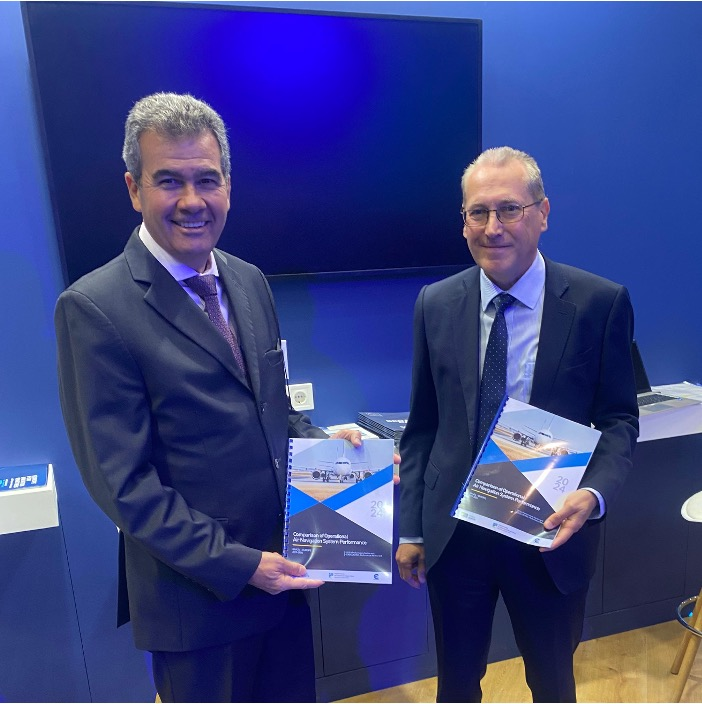
\includegraphics[width=0.55\linewidth,height=\textheight,keepaspectratio]{./figures/DGCEA-PRC.jpg}
\end{center}

\bookmarksetup{startatroot}

\chapter*{Executive Summary}\label{executive-summary}
\addcontentsline{toc}{chapter}{Executive Summary}

\markboth{Executive Summary}{Executive Summary}

The Performance Section of the Brazilian Department of Airspace Control
and the Performance Review Unit of EUROCONTROL jointly developed this
fourth edition of the Brazil-Europe comparison of Air Navigation System
Performance. This edition of the bi-regional report builds on the
previous comparison reports using commonly agreed metrics and
definitions to compare, understand, and improve the performance of air
navigation services. This report and previous editions are available via
the web-portals of both organisations:

\begin{itemize}
\tightlist
\item
  \url{https://ansperformance.eu/global/brazil} or
\item
  \url{https://performance.decea.mil.br/}.
\end{itemize}

This edition expands on the previous comparisons of the Brazilian and
European air navigation systems by focussing on the observed performance
post COVID, extending the time frame, and incorporating additional
analyses. For example, a more detailed characterisation of the Brazilian
and European network is included. With the recent deployment of
point-merge, operations at Sao Paulo Guarulhos and Lisbon are studied
and an initial characterisation is provided. On the center level, this
edition also looks into comparing Curitiba and Lisbon ACC. These
focussed topics allow to address discussions about performance benefits
and may help to highlight the differences between the operations in both
regions.

The report focuses on a subset of the eleven Key Performance Areas
identified by the ICAO Global Air Navigation Plan, in particular
Predictability, Capacity and Efficiency.

\begin{figure}[H]

\centering{

\includegraphics[width=0.6\linewidth,height=\textheight,keepaspectratio]{./figures/scope-KPA-and-KPI.png}

}

\caption{\label{fig-scope-KPAs-KPIs}Key Performance Areas addressed in
this edition}

\end{figure}%

The comparison shows similarities and differences in the air navigation
service provision and observed performance in both regions. Major
take-aways of this report include:

\begin{itemize}
\tightlist
\item
  The close collaboration between DECEA and EUROCONTROL is highlighted
  sharing insights and experiences with the international aviation
  communities, thus assisting in advancing ATM performance management
  worldwide.
\item
  While the observed performance levels in both regions differ,
  similarities and understood differences support more targeted
  discussions on operational concepts. With Europe closing in on
  pre-pandemic traffic levels and Brazil now consistently observing
  demand above the pre-pandemic level, this edition also forms the
  reference for future iterations.
\item
  Regarding punctuality, unique trends were evident in both regions, not
  solely attributable to the extent of traffic resurgence. In Brazil, a
  consistently higher proportion of flights arrived significantly early,
  a pattern largely unaffected when comparing previous years.
  Conversely, the documented challenges of European airports in coping
  with the recovering traffic demand and the record high of network
  constraints in 2023 and 2024 impact the robustness of the schedule.
\item
  Overall, Europe showed a higher level of throughput as the higher
  traffic numbers and constraints require a higher level of pressure on
  the infrastructure. Nonetheless, the constraints of reaching
  pre-pandemic traffic levels will require attention in terms of
  increasing efficiency and reducing capacity constraints with future
  growth. Brazil may benefit from increasing their stance and
  maintaining current performance levels with the anticipated growth of
  traffic.
\item
  This report took a first stab at characterising the regional networks
  for future topic-centric amendments. This will allow to drive future
  topic studies and provide essential context. As an initial
  topic-related study, a closer look was taken at two point merge
  implementations in Brazil and Europe that show different performance
  outcomes. This is complemented by providing a first look at the
  operational context of two centres, i.e., Curitiba and Lisbon. This
  edition helped to frame the work and identify a set of future research
  questions.
\end{itemize}

This report will be updated throughout the coming years under the
umbrella of the DECEA-EUROCONTROL memorandum of cooperation. It is also
planned to establish a web-based rolling monitoring updated on a regular
basis.

Future editions will complement the data time series and support the
development of further use-case analyses. The lessons learnt of this
joint project will be coordinated with the multi-national Performance
Benchmarking Working Group (PBWG) and the ICAO GANP Study sub-group
concerned with the further development of the GANP Key Performance
Indicators (KPIs).

\bookmarksetup{startatroot}

\chapter{Introduction}\label{introduction}

\pagenumbering{arabic}
\setcounter{page}{1}

\section{Background}\label{background}

Air transportation is a key economic driver in Brazil and Europe. Both
regions share the political goal of a performance-based approach to
foster the continual growth and efficiency of air transport. It is
recognised that Air Navigation Services (ANS) play a critical role in
terms of limiting the constraints on airspace user operations.
Accordingly, the analysis and regional comparison of operational ANS
performance informs about trends over time, the success of change
implementation, and potential performance benefit pools for future
exploitation.

With a view to a tighter collaboration between Brazil and Europe, DECEA
and EUROCONTROL signed a cooperation agreement in 2015. This agreement
encompasses various activities, most notably the cooperation and joint
initiatives in the domain of operational performance benchmarking of
ANS.

The close technical collaboration of the Performance Section of DECEA
and EUROCONTROL's Performance Review Unit comprises the further
development and validation of proposed ICAO GANP indicators, regular
performance related data exchange, and the production of regional or
multi-regional performance reports. An essential part of this work
entails the identification and validation of comparable data sources,
the development of a joint data preparatory process, and supporting
analyses to produce this report or contribute to the aforementioned
international activities.\\
This report represents the fourth edition of a jointly developed
comparison report providing insights into the observed operational
performance in Brazil and Europe.

\section{Performance Areas}\label{performance-areas}

Establishing a set of shared definitions and a mutual understanding is
essential to facilitate comparisons and operational benchmarking
activities. Therefore, the work presented in this report is rooted in
prior work conducted by ICAO, other regional or multi-regional
operational benchmarking initiatives (e.g., PBWG \footnote{The
  Performance Benchmarking Working Group (PBWG) comprises participants
  from Brazil (DECEA), China (CAA-OSC), Japan (JCAB), Singapore (CAA),
  Thailand (AEROTHAI), United States (FAA-ATO), and EUROCONTROL.}), and
practices within various regional or organisational settings.

The key performance indicators (KPIs) utilised in this study have been
developed through a rigorous process that integrates the best available
data from both the DECEA Performance Section and PRU. It is important to
note that the comparative analysis in this iteration of the report does
not encompass all eleven Key Performance Areas (KPA) as presented in
Figure~\ref{fig-scope-KPAs-KPIs}.

From an indicator perspective, the DECEA Performance Section and PRU
have reached a consensus to concentrate on operational benchmarking and
aligning their efforts with the performance indicators proposed by ICAO
in conjunction with the update of the Global Air Navigation Plan (GANP).
Discussions are on-going, and future work may also include aspects of
cost-effectiveness.

\section{Geographical Scope}\label{geographical-scope}

This report's geographical focus encompasses Brazil and Europe.

Airspace control in Brazil is a fully integrated civil-military
operation. The Brazilian Air Force is responsible for air defence and
air traffic control functions. This ensures air traffic safety while
contributing to military defence efforts. Within this framework, the
Department of Airspace Control (DECEA) operates as a governmental entity
under the authority of the Brazilian Air Force Command. DECEA plays a
pivotal role in coordinating and furnishing human resources and
technical equipment to all air traffic service units operating within
the Brazilian territory.

DECEA is the cornerstone of the Brazilian Airspace Control System
(SISCEAB). The department provides air navigation services for the vast
airspace jurisdiction covering 22 million square kilometres, including
oceanic areas. The Brazilian airspace is further divided into five
Flight Information Regions (FIR) and the areas of responsibility of
these integrated Centres for Air Defence and Air Traffic Control
(CINDACTA) are depicted in Figure~\ref{fig-BRA-airspace}.

\begin{figure}[H]

\centering{

\includegraphics[width=3.71in,height=\textheight,keepaspectratio]{./figures/BRAZIL_CINDACTA_AND_CRCEA.png}

}

\caption{\label{fig-BRA-airspace}Brazilian Airspace Structure/FIRs
(CINDACTAs)}

\end{figure}%

The CINDACTAs merge civilian air traffic control with military air
defence operations. In addition to the CINDACTAs, there's the Regional
Center of Southeast Airspace Control (CRCEA-SE). The latter is tasked
with managing air traffic in the densely congested terminal areas of São
Paulo and Rio de Janeiro.

\begin{figure}[H]

\centering{

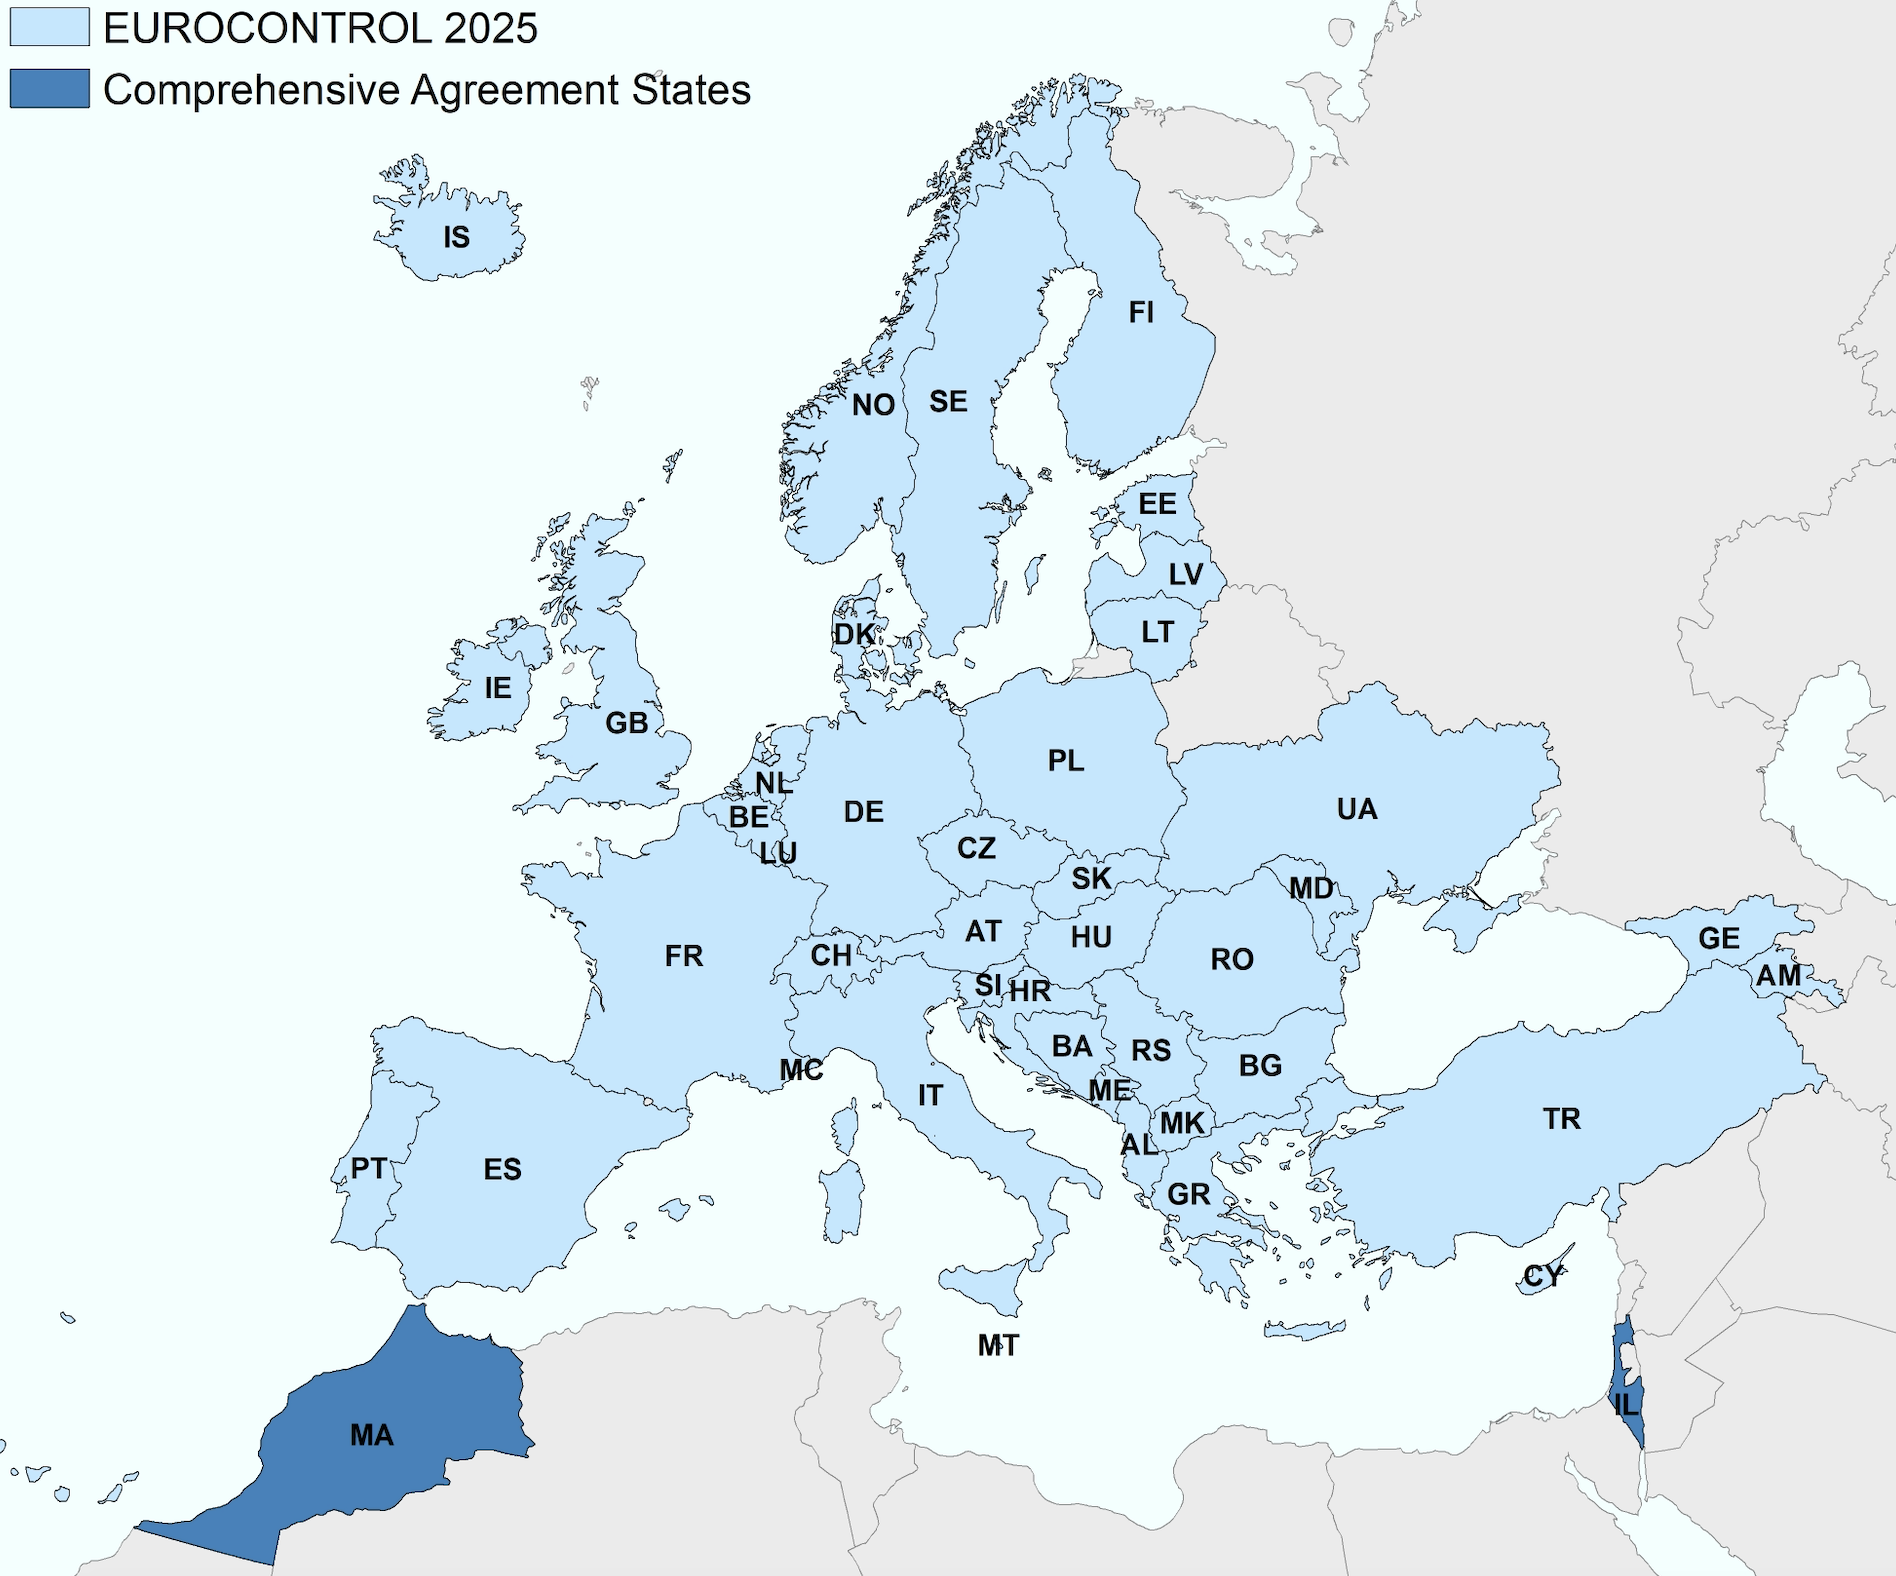
\includegraphics[width=0.9\linewidth,height=\textheight,keepaspectratio]{./figures/Europe-ECTRL.png}

}

\caption{\label{fig-EUR-airspace}European Airspace and EUROCONTROL
Member States}

\end{figure}%

In this report, Europe, i.e.~the European airspace, is defined as the
area where the 42 EUROCONTROL member states provide air navigation
services, excluding the oceanic areas and the Canary islands (c.f.
Figure~\ref{fig-EUR-airspace}). In 2016, EUROCONTROL signed a
comprehensive agreement with Israel and Morocco. Both comprehensive
agreement States will successively be fully integrated into the working
structures of EUROCONTROL, including performance monitoring, in the
coming years. Within this report, these states are included in the
reported network traffic volumes.

EUROCONTROL is an inter-governmental organisation working towards a
highly harmonised European air traffic management system. In general,
air traffic services are provided by - predominantly national or local -
air navigation service providers entrusted by the different EUROCONTROL
member states. Dependent on the local and national regimes, there is a
mix of civil and military service providers, and integrated service
provision.\\
The Maastricht Upper Area Control Center is operated by EUROCONTROL on
behalf of 4 States (Netherlands, Belgium, Luxemburg, and Germany). It is
the only multi-national cross-border air traffic service unit in Europe
at the time being. Across Europe a number of cross-border arrangements
are in place. Given the European context and airspace structure, the
European area comprises 37 ANSPs with 62 en-route centres and 16
stand-alone Approach Control Units (i.e.~totalling 78 air traffic
service units).

Europe employs a collaborative approach to managing and servicing
airspace and air traffic. This includes the integration of military
objectives and requirements which need to be fully coordinated within
the ATM System. A variety of coordination cells/procedures exists
between civil air traffic control centres and air defence units
reflecting the local practices. Many EUROCONTROL member states are
members of NATO and have their air defence centres / processes for
civil-military coordination aligned under the integrated NATO air
defence system.

Further details on the organisation of the regional air navigation
systems in Brazil and Europe will be provided in Section 2.1.

\subsection{Study Airports}\label{study-airports}

As concerns airport-related operational air navigation performance, this
edition of the comparison report addresses the performance at a set of
selected airports. These airports represent the top-10 or most relevant
airports in terms of IFR movements in both regions and allow to make
meaningful comparisons.\\
In Brazil, the selected airports play a significant role for the
national and regional connectivity, including the major hubs for
international air traffic. These study airports have consolidated
systems and structured processes for data collection in support of this
comparison report.\\
For the European context, the study airports comprise the busiest
airports in several states exhibiting a mix of national, regional, and
international air traffic. These airports are also characterised by
varying operational constraints that make them excellent candidates for
an international comparison. All of these airports are subject to the
performance monitoring under the EUROCONTROL Performance Review System
and provide movement related data on the basis of a harmonised data
specification.

Figure~\ref{fig-scope-airports} provides an overview of the location of
the chosen study airports within both regions. The airports are also
listed in Table~\ref{tbl-scopetable}.

\begin{longtable}{ll}

\caption{\label{tbl-scopetable}List of study airports for the Brazil /
Europe operational ANS performance comparison}

\tabularnewline

\toprule
Brazil & Europe \\ 
\midrule\addlinespace[2.5pt]
Brasília (SBBR) & Amsterdam Schiphol (EHAM) \\ 
São Paulo Guarulhos (SBGR) & Paris Charles de Gaulle (LFPG) \\ 
São Paulo Congonhas (SBSP) & London Heathrow (EGLL) \\ 
Campinas (SBKP) & Frankfurt (EDDF) \\ 
Rio de Janeiro S. Dumont  (SBRJ) & Munich (EDDM) \\ 
Rio de Janeiro Galeão (SBGL) & Madrid (LEMD) \\ 
Belo Horizonte Confins (SBCF) & Lisbon (LPPT) \\ 
Salvador (SBSV) & Barcelona (LEBL) \\ 
Porto Alegre (SBPA) & London Gatwick (EGKK) \\ 
Curitiba (SBCT) & Zurich (LSZH) \\ 
\bottomrule

\end{longtable}

\begin{figure}[H]

\centering{

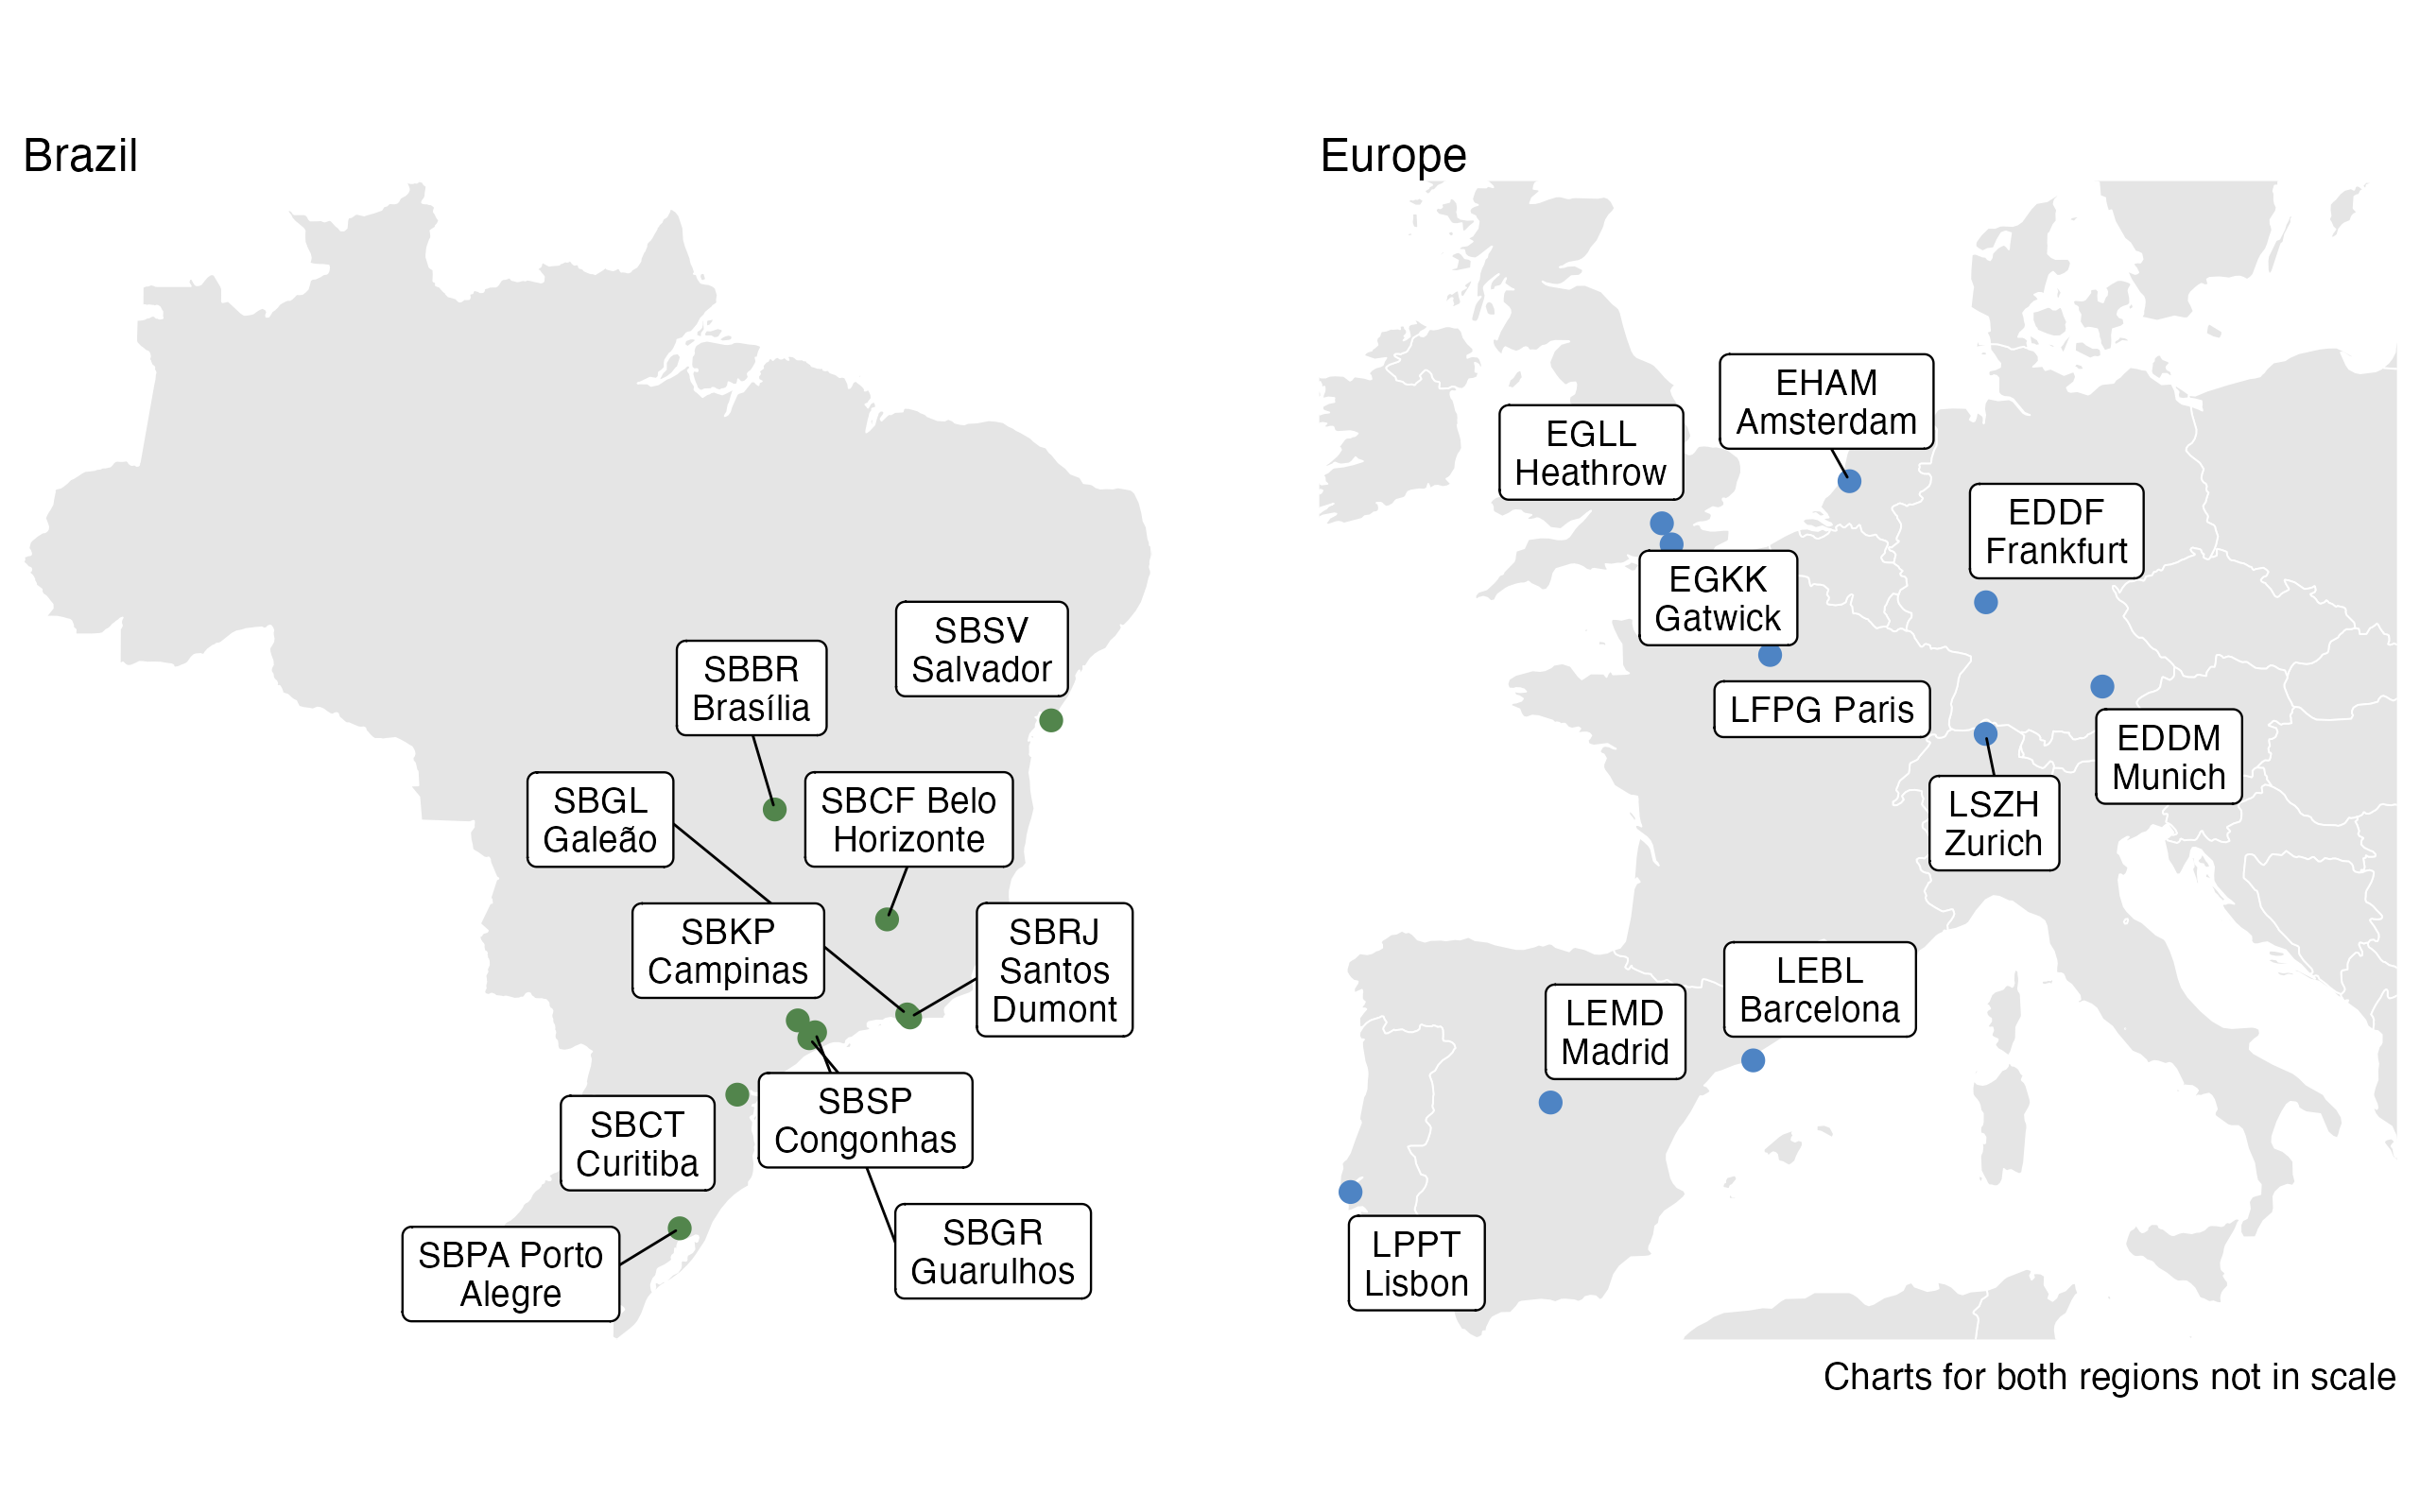
\includegraphics[width=0.9\linewidth,height=\textheight,keepaspectratio]{./figures/_scope-airports-map.png}

}

\caption{\label{fig-scope-airports}Study airports of Brazil/Europe
Comparison}

\end{figure}%

\subsection{Temporal Scope}\label{temporal-scope}

This report focuses on the period from January 2019 to December 2024
with a focus on the post-pandemic years. This report continues to build
a timeline with comparable data to be augmented in future editions.

Throughout the report, summary statistics will be given with reference
to calendar years of this comparison study unless highlighted
specifically.

\section{Data Sources}\label{data-sources}

The nature of the performance indicator requires the collection of data
from different sources. DECEA Performance Section and PRU investigated
the comparability of the data available in both regions, including the
data pre-processes, data cleaning and aggregation, to ensure a
harmonised set of data for performance comparison purposes.

DECEA mainly uses data from the tower systems of the main airports as a
data source for performance studies. The control tower system collects
and provides data for each landing and take-off operation automatically.
This edition blended ANAC (Brazilian CAA) official and public data with
DECEA's data to increase precision for specific indicators, adding a
pre-processing phase to the data analytical work. The provided data
include such items as the times of operations, gate entry and exit, and
flight origin and destination.

Within the European context, PRU has established a variety of
performance-related data collection processes. For this report the main
sources are the European Air Traffic Flow Management System (ETFMS
\footnote{Enhanced Traffic Flow Management System}) complemented with
airport operator reported data. These sources are combined to establish
a flight-by-flight record. This ensures consistent data for arrivals and
departures at the chosen study airports. The data is collected on a
monthly basis and typically processed for the regular performance
reporting under the EUROCONTROL Performance Review System and the Single
European Sky Performance and Charging Scheme (EUROCONTROL 2019).

\section{Structure of the Report}\label{structure-of-the-report}

This third edition of the Brazil-Europe comparison report is organised
as follows:

\begin{itemize}
\tightlist
\item
  \textbf{Introduction} -- overview, purpose and scope of the comparison
  report; short description of data sources used;
\item
  \textbf{Air Navigation System Characteristics} -- high-level
  description of the two regional systems, i.e.~areas of responsibility,
  organisation of ANS, and high-level air navigation system
  characteristics;
\item
  \textbf{Traffic Characterisation} -- network level and airport level
  air traffic movements; peak day demand, and fleet composition observed
  at the study airports;
\item
  \textbf{Predictability} observed arrival and departure punctuality;
\item
  \textbf{Capacity and Throughput} assessment of the declared capacity
  at the study airports and the observed throughput, including runway
  system utilisation comparing achieved peak throughput to the declared
  capacity;
\item
  \textbf{Efficiency} analysis of taxi-in, taxi-out, and terminal
  airspace operations
\item
  \textbf{Topic Studies} presents a high-level view on the use of point
  merge operations at two study airports, and a center-level
  characterisation; and
\item
  \textbf{Conclusions} summary of this report and associated
  conclusions; and next steps.
\end{itemize}

\bookmarksetup{startatroot}

\chapter{Air Navigation System
Characterisation}\label{air-navigation-system-characterisation}

This section presents key characteristics of the air navigation systems
of Brazil and Europe. In broad strokes, the provision of air navigation
services in both regions relies on similar operational concepts,
procedures, and supporting technology. Nonetheless, there are several
distinctions between the two systems, which help to account for the
similarities and differences in key performance indicators documented in
this report.

\section{Organisation of Air Navigation
Services}\label{organisation-of-air-navigation-services}

One of the major differences between the air navigation systems of
Brazil and Europe is the respective organisational structure. In Brazil,
a single entity serves as the primary air navigation services provider,
i.e.~the Department of Airspace Control (DECEA). In contrast, in Europe,
each member state has delegated the responsibility for service provision
to either national or local providers.

DECEA holds the vital role of overseeing all activities related to the
safety and efficiency of Brazilian airspace control. Its mission
encompasses the management and control of all air traffic within the
sovereign Brazilian airspace, with a significant emphasis on
contributing to national defence efforts. To achieve this, DECEA
operates a comprehensive and fully integrated civil-military system.

In 2021, a public company, NAV Brasil, was created to take over some
facilities that were linked to an older airport infrastructure provider
company in Brazil (INFRAERO). Today, NAV Brasil has 1698 employees in 44
different units, providing aerodrome control services, non-radar
approach, meteorology and aeronautical information for the respective
locations. Despite serving a significant number of air transport
movements, NAV Brasil does not plan to establish radar facilities or
provide en-route services.

The Brazilian airspace, covering an area of approximately 22 million
square kilometres (8.5 million square nautical miles of non-oceanic
airspace), is divided into five Flight Information Regions. These
regions are further subdivided and managed by five Area Control Centers
(ACC), 57 Tower facilities (TWR), one digital tower (D-TWR), 41 Approach
Units (APP) and 79 AFIS/Remote-AFIS.

The non-oceanic airspace in Europe covers an area of 11.5 million square
kilometres. When it comes to the provision of air traffic services, the
European approach involves a multitude of service providers, with 37
distinct en-route Air Navigation Service Providers (ANSPs), each
responsible for different geographical regions. These services are
primarily organised along state boundaries and associated FIR borders,
with a number of limited cross-border agreements in place between
adjacent airspaces and air traffic service units.\\
A noteworthy exception to this predominantly national approach is the
Maastricht Upper Area Control, which represents a unique multinational
collaboration offering air traffic services in the upper airspace of
northern Germany, the Netherlands, Belgium, and Luxembourg.

Civil-military integration levels across European countries vary. Within
the European context, the central coordination of Air Traffic Flow
Management (ATFM) and Airspace Management (ASM) is facilitated by the
Network Manager. The design of airspace and related procedures is no
longer developed and implemented in isolation in Europe. Inefficiencies
in the design and utilisation of the air route network are recognised as
contributing factors to flight inefficiencies in the region. Therefore,
as part of the European Union's Single European Sky initiative, the
Network Manager is tasked with developing an integrated European Route
Network Design. This is achieved through a Collaborative Decision-Making
(CDM) process involving all stakeholders.

Another critical responsibility of the Network Manager is to ensure that
air traffic flows do not exceed the safe handling capacity of air
traffic service units while optimising available capacity. To accomplish
this, the Network Manager Operations Centre (NMOC) continuously monitors
the air traffic situation and proposes flow management measures through
the CDM process in coordination with the respective local authorities.
This coordination typically occurs with the local Flow Management
Positions (FMP) within the respective area control centres.
Subsequently, the NMOC implements the relevant flow management
initiatives as requested by the authorities or FMPs.

\section{High Level System
Comparison}\label{high-level-system-comparison}

Table~\ref{tbl-HLC} summarises the key characteristics of the Brazilian
and European air navigation system for 2024. Comparing the high-level
numbers, Brazil observed a steady increase in the number of Air Traffic
Controllers (ATCOs) compared to 2019 (e.g.~2023 vs 2019: 17.6\%, 2024 vs
2019: 24.4\%). In contrast, the European system showed only a mild
increase in total ATCOs in service following the strong reduction during
the pandemic in terms of work force. The different behaviour suggests a
difference in work force flexibility between the systems. Brazil reacted
swiftly to the increase of air traffic ranging at 21.4\% higher than in
2019. Europe has seen a mild modulation of ATCO numbers with the annual
traffic in 2024 ranging about 4\% below the 2019 level.\\
This may be partly explained by the fact that DECEA shares part of the
structure used in basic training with other Air Force training
processes. This leads to a more centralised and rigid process, in which
abrupt reactions in hiring planning are unwanted due to the lengthy
process of calling for candidates according to Brazilian laws related to
public service jobs. In Europe, there exists a mix of organisational
models and labour contracts ranging from public service to fully
commercial organisation. Thus, European providers tend to react more
conservative to anticipated changes in air traffic demand.

\begin{table}

\caption{\label{tbl-HLC}High Level Comparison 2024}

\centering{

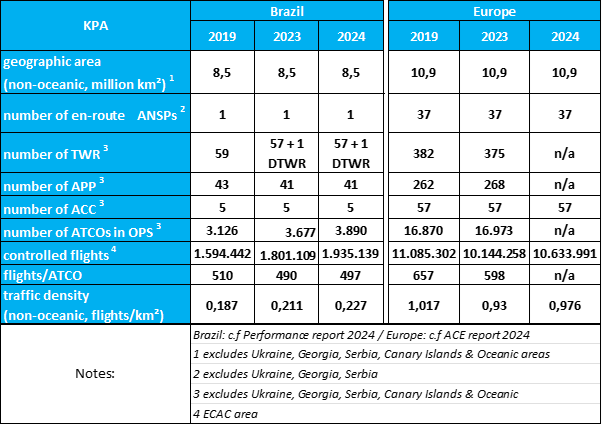
\includegraphics[width=0.95\linewidth,height=\textheight,keepaspectratio]{./figures/HLC-table1.png}

}

\end{table}%

Another key difference affecting performance in both regions for this
report is the development of air traffic demand. Unlike in Europe, it is
interesting to note that Brazil ended 2022 already servicing air traffic
movements above the pre-pandemic level. There is a continual increase in
air traffic in Brazil accounting now for 21,4\% of more traffic than in
2019. Overall, the volume of air traffic also rebounded in Europe. At
the end of 2023, the level reached about 90\% of the pre-pandemic air
traffic, and with 2024 the gap is closing to about 96\%. These recovery
numbers are impacted by the geo-political developments. Due to the
Russian invasion of Ukraine, a certain share of flights is currently
banned to operate to/from Europe.

Both regions operate with similar operational concepts, procedures and
supporting technology. Considering the non-oceanic dimension of the
airspace, Brazil services an area about 22\% smaller than Europe.
Brazil, with lower traffic density related to airspace, finds probably a
more challenging cost-benefit ratio to maintain communication coverage
and surveillance for regions with low-traffic. The higher traffic
density in Europe may cross all aspects of flight management. In
particular, the European region faces more considerable challenges in
coordinating efforts to address operational constraints and service the
current demand.

\section{Network Characterisation}\label{network-characterisation}

To address the changes in air traffic and develop a better understanding
of the nature of the air transportation network, this report expands the
characterisation of the network.
Figure~\ref{fig-apt-rank-comparison-2024} depicts the cumulative share
of departures from airports in both regions.

\begin{figure}[H]

\centering{


\includegraphics[width=0.9\linewidth,height=\textheight,keepaspectratio]{02-system-overview_files/figure-pdf/fig-apt-rank-comparison-2024-1.pdf}

}

\caption{\label{fig-apt-rank-comparison-2024}Airport Rank Comparison
2024}

\end{figure}%

Table~\ref{tbl-HLC} lists the overall serviced traffic in both regions.
In 2024 Brazil observed just under a fifth (18.2\%) of the traffic
handled in Europe. With overflights representing a small share of the
traffic in both regions, Figure~\ref{fig-apt-rank-comparison-2024}
focusses on the aerodrome movements considering all observed departures.
The distribution of air traffic in Brazil confirms that most flights are
concentrated in a small number of airports. Traffic in Europe operates
from a larger number of aerodromes. For example, in 2024, the 10 busiest
airports in Brazil handled 61\% of all departing flights whereas in
Europe, the top 10 airports account for 19\% of all departures. The
spread in shares remains broadly constant up to the 50th rank of all
departures and narrows to 30\% with the top 100 airports in both
regions. The latter marking 97\% of all departures in Brazil and 67\% in
Europe.

The latest edition of Brazil's Annual Performance Report (it can be
found on http://performance.decea.mil.br) reflects this reality. It now
includes 100 airport locations instead of only the top 34, ensuring that
almost all flights are included in the analysis. This distribution shows
that many aerodromes operate with low traffic volumes. Because of that,
it is important to study alternative ways to provide air traffic
services.

In Brazil, the Aerodrome Flight Information Service (AFIS) is an
effective strategy to ensure safety at locations where the traffic does
not justify the installation of a control tower (TWR). This service,
usually provided via radio telephony only, gives essential information
to pilots, helping to use resources efficiently and keeping operations
safe. Since 2016, Brazil has been expanding the use of remote AFIS units
(R-AFIS), especially in strategic areas like the Amazon region. These
services are provided from ACCs (Area Control Centers), which means they
don't need dedicated local infrastructure. Also, in 2024, demand for air
traffic services continued to grow. This shows the need to review and
improve how services are organized in Brazil. Expanding the use of the
AFIS model in strategic areas may be a cost-effective and safe way to
meet future needs and make better use of SISCEAB's resources.

The more spread-out distribution in Europe showcases the historical
development of the European network. The traditional focus on national
hubs and carriers resulted in the development of a higher number of
major aerodromes (typically servicing the capital, major metropoles, or
economic centers) interconnecting with other national hubs across the
continent. There exists a mix of the organisation of smaller operations
in Europe. Dependent on the national or local setup, the resources of
the national service provider are often complemented by local service
providers. Thus, the provision of services varies between smaller manned
towers and remotely provided FIS functions provided by nearby ACCs. This
includes instrument procedures to approach (and depart) from an
uncontrolled aerodrome. Given this mix of organisation and funding in
Europe, no consolidated pan-European data was available to specifically
account for local AFIS services. Across Europe, there is an interest in
consolidating aerodrome control services at important low frequency
sites through the deployment of digital remote tower operations. This
ranges from site specific remote tower operations (e.g.~Cork/Ireland) to
a multi-remote tower center (e.g.~Stockholm/Sweden, Bodo/Norway)
servicing multiple airports simultaneously.

While the view on the concentration of air traffic provides first
insights, the level of connectivity is not immediately identifiable.

\begin{figure}

\begin{minipage}{0.50\linewidth}

\begin{figure}[H]

\centering{

\pandocbounded{
\includegraphics[keepaspectratio]{02-system-overview_files/figure-pdf/fig-share-intnl-regional-1.pdf}}

}

\caption{\label{fig-share-intnl-regional}Share of international and
regional/domestic traffic in 2024}

\end{figure}%

\end{minipage}%
%
\begin{minipage}{0.50\linewidth}
Figure~\ref{fig-share-intnl-regional} shows the distribution of
regional/domestic and international departures. For both regions we
observe a share of less than 12\% of serviced traffic are flights
operating to and from the regions. The majority of flights operate
within the region, i.e., within the domestic Brazilian network and
conversely the European network spanning across EUROCONTROL Member
States.\end{minipage}%

\end{figure}%

\begin{figure}

\begin{minipage}{0.50\linewidth}

\begin{figure}[H]

\centering{

\pandocbounded{
\includegraphics[keepaspectratio]{02-system-overview_files/figure-pdf/fig-share-intnl-regions-1.pdf}}

}

\caption{\label{fig-share-intnl-regions}Share of destinations in 2024}

\end{figure}%

\end{minipage}%
%
\begin{minipage}{0.50\linewidth}
From an international perspective both regions are interconnected
differently. Figure~\ref{fig-share-intnl-regions} sees a spread of the
international traffic to other regions. Traffic from Brazil to Europe
(i.e., Eurocontrol Member States) accounts for just under 2\% of the
total traffic volume in Brazil. Connections to other Southern America
states represent the major international destinations accounting for
about 5\%. Europe has a shallow share of flights going to Southern
America, including Brazil. The Middle East, Northern America, and Africa
represent the biggest international markets ranging between 2.3-3.3\% of
all departures in Europe.\end{minipage}%

\end{figure}%

\begin{figure}[H]

\centering{

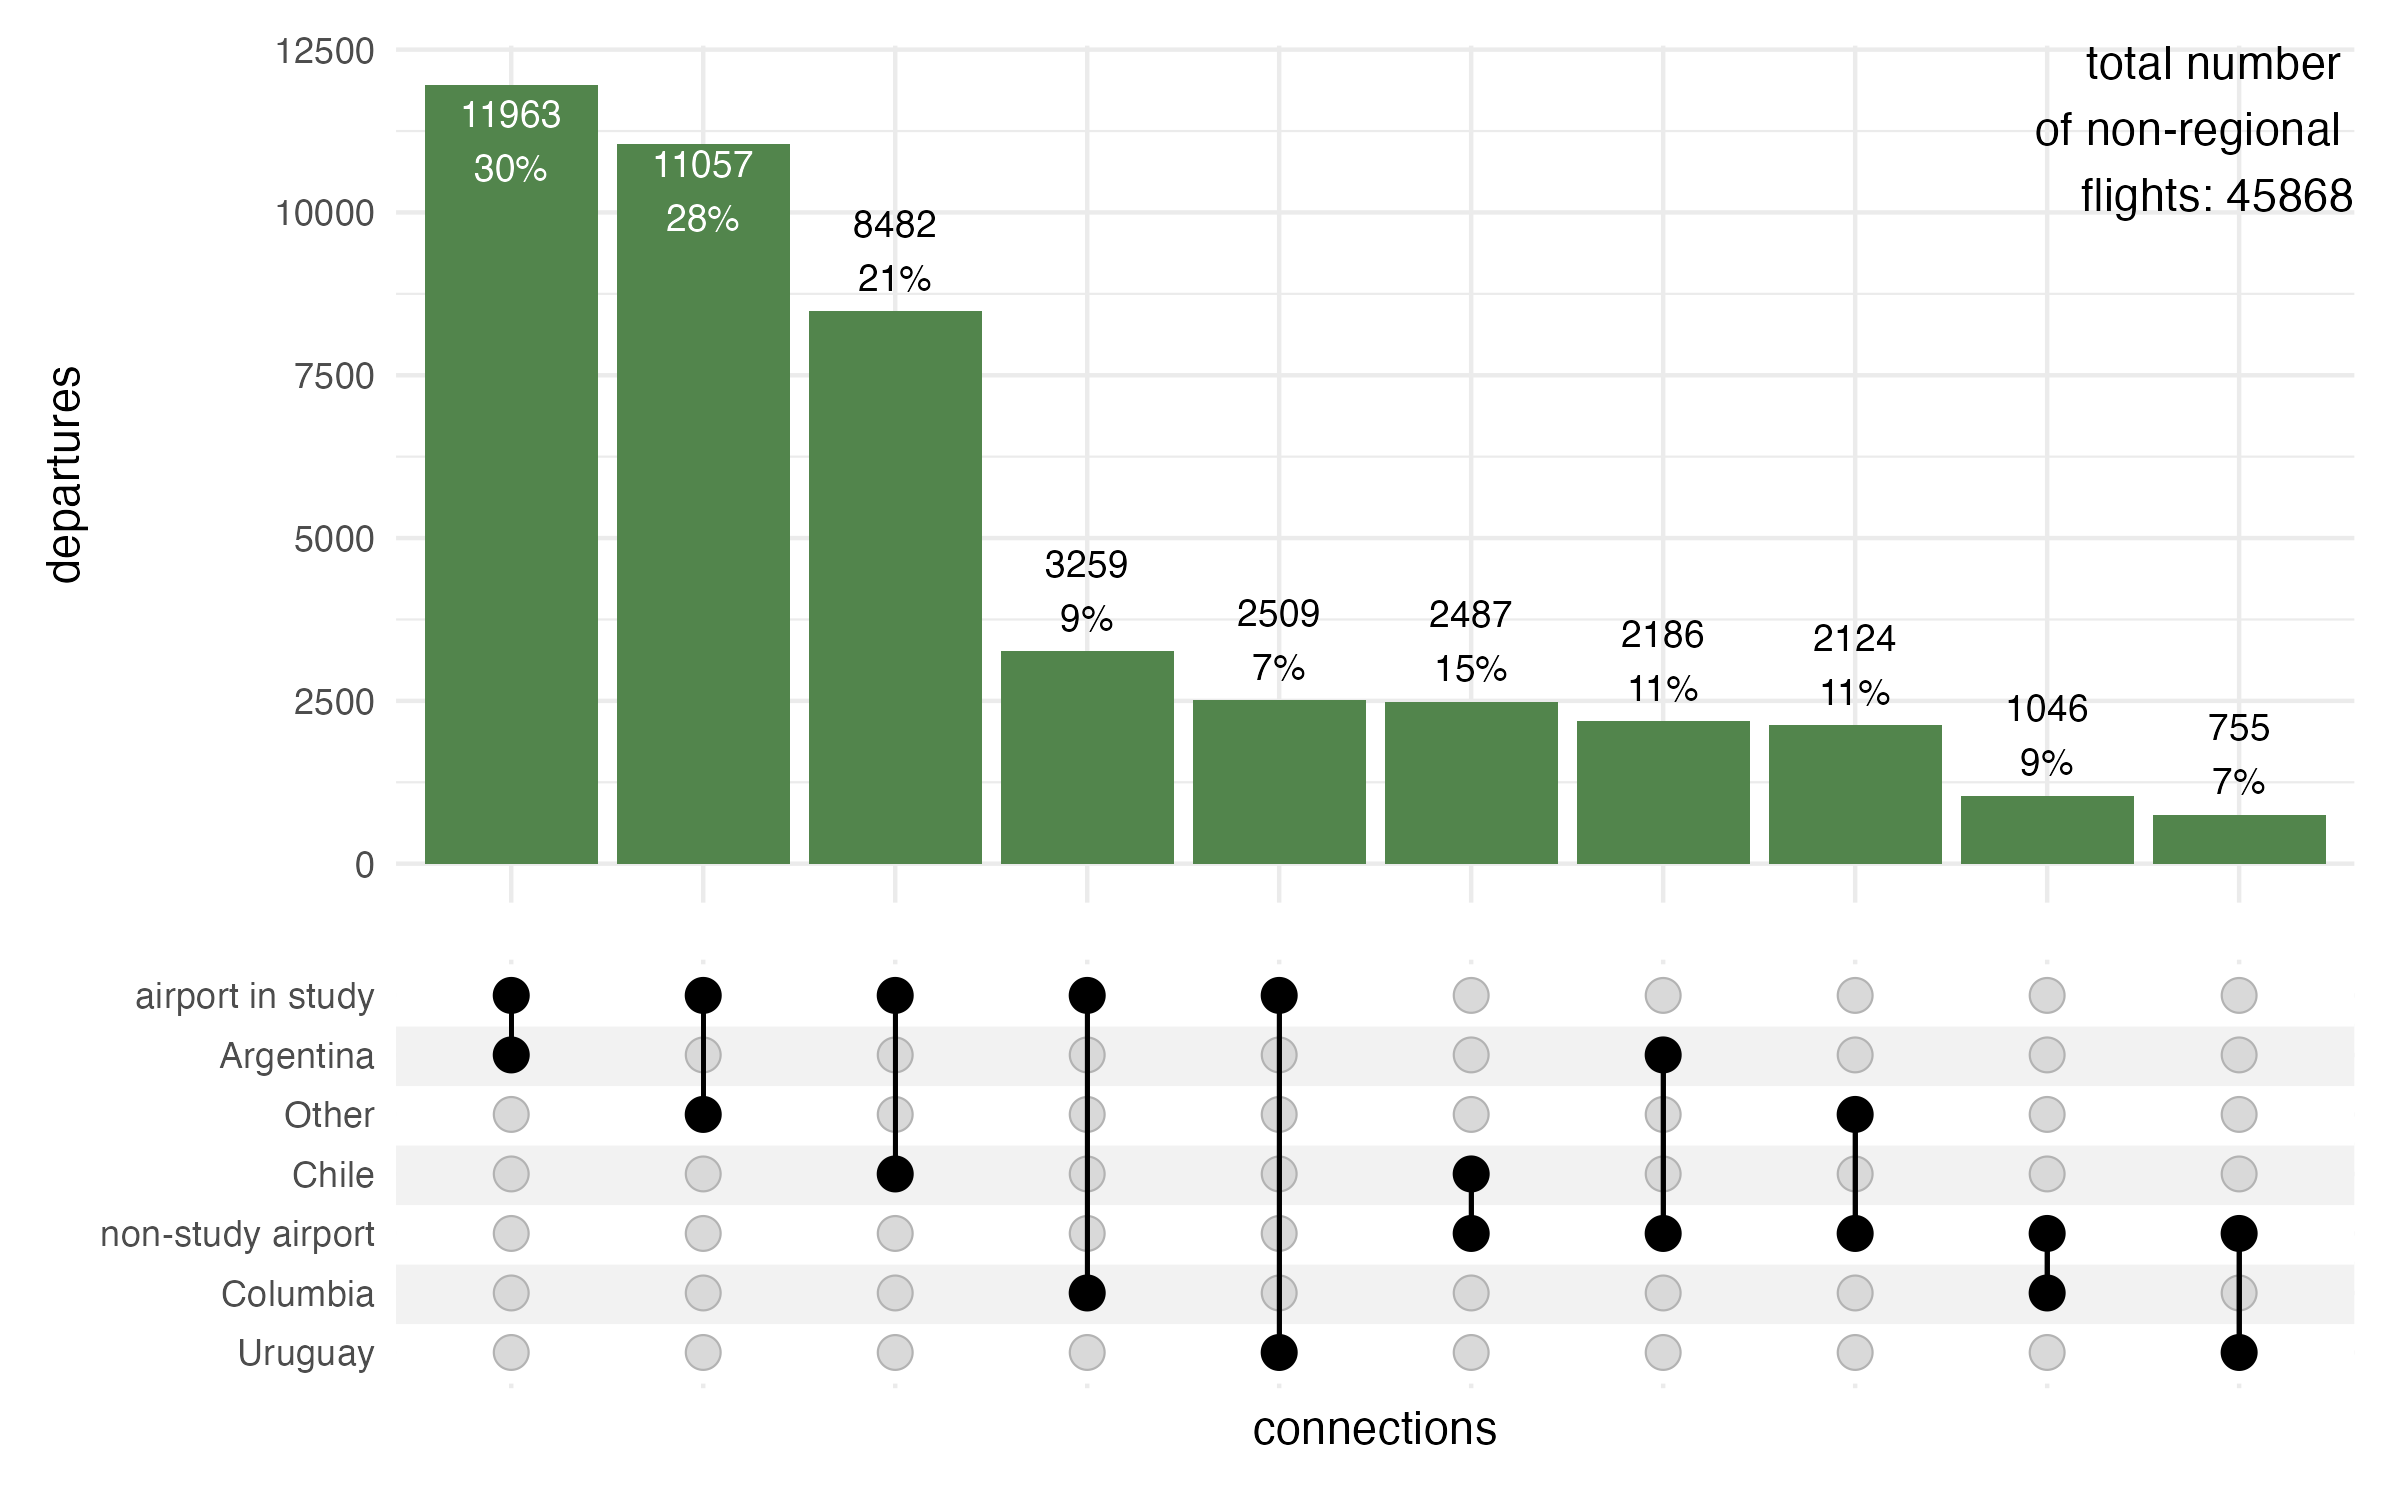
\includegraphics[width=0.9\linewidth,height=\textheight,keepaspectratio]{./figures/BRA-upset-national-connections.png}

}

\caption{\label{fig-BRA-upset-connection}Connections to adjacent
countries}

\end{figure}%

With Figure~\ref{fig-BRA-upset-connection} we observe just under 46.000
flights in 2024 operated to adjacent countries in South America. A
strong segment of the market represents flights to/from Argentina and
Chile accounting for about half of the flights departing from the
airports in this study. Accordingly, flights to Colombia and Uruguay
from the study airports account for a smaller fraction, and there is a
multitude of other connections to South America and the Caribbean.
Flights operating from airports not included in this study account for
smaller shares. This confirms the selection of the study airports for
Brazil, as the major airports handle most of the pan-regional traffic
with a strong connection to Argentina and Chile.

\begin{figure}[H]

\centering{

\pandocbounded{
\includegraphics[keepaspectratio]{02-system-overview_files/figure-pdf/fig-BRA-EUR-connections-parallel-1.pdf}}

}

\caption{\label{fig-BRA-EUR-connections-parallel}Connections between the
study regions in 2024}

\end{figure}%

Figure~\ref{fig-BRA-EUR-connections-parallel} shows the connections
between Europe and Brazil in 2024. Individual connections of less than
90 flights per year are aggregated into an ``other'' group. These
largely reflect specific individual flights (e.g.~State flights, special
cargo operations), and only contribute to a small extent to the overall
traffic between both regions.\\
Guarulhos (SBGR) and Lisbon (LPPT) are the main airports for
connectivity between both regions. Due to its prominent role, this
edition considers operations at LPPT in a more prominent manner.

Future work may highlight to what extent resources within both regions
are bound to establishing basic connectivity and what type of services
are provided to accommodate the demand. Further research can explore how
both regions can maximise installed capacity, benefit from novel
operational or technical concepts, and suggest improvements for ANS
provision.

\section{Regional Approach to Operational Performance
Monitoring}\label{regional-approach-to-operational-performance-monitoring}

The previous report detailed the historic setup of the performance
monitoring systems in Brazil and Europe.

The implementation of the performance-based approach is not a
fundamental new activity in Europe. The Performance Review Commission
(PRC) was established within EUROCONTROL in 1998 aiming to establish and
implement an independent European air traffic management (ATM)
performance review capability in response to the European Civil Aviation
Conference (ECAC) Institutional Strategy. The main goal of the PRC is to
offer impartial advice on pan-European ATM performance to EUROCONTROL's
governing bodies. Supported by the Performance Review Unit (PRU), the
PRC conducts extensive research, data analysis, and consultations to
provide objective insights and recommendations. EUROCONTROL's
performance review system, a pioneering initiative in the late 1990s,
has influenced broader forums like ICAO's global performance approach
and the Single European Sky (SES) performance scheme. Collaborating
internationally, particularly with ICAO, the PRC aims to harmonise air
navigation practices. The PRC produces annual reports (ACE and PRR) and
provides operational performance monitoring through various data
products and online tools. Continuous efforts are made to expand the
online reporting for stakeholders and ensure access to independent
performance data for informed decision-making.

It is noteworthy to recall that DECEA, influenced by ICAO publications,
embraced a performance-based approach, notably advancing the national
state-of-the-art in collaboration with EUROCONTROL. Beginning with the
SIRIUS Brazil Program in 2012, DECEA faced challenges defining metrics,
but made significant progress after signing a Cooperation Agreement with
EUROCONTROL in 2015. DECEA published crucial documents for ICAO's Global
Air Navigation Plan, prompting an organisational transformation and
adaptation of practices. Establishing the ATM Performance Section in
2019, akin to EUROCONTROL's PRU, DECEA accelerated the build-up of
expertise in operational performance monitoring. This culminated in the
publication of the first Brazilian ATM Performance Plan for 2022-2023.
Actively fostering an open culture of knowledge-sharing within South
America, DECEA engaged in workshops and seminars, and inviting
EUROCONTROL for collaboration.

Finally, it should be noted that the recurrent use of indicators by
EUROCONTROL and DECEA and the close technical collaboration taking place
during the analysis periods for joint conclusions enrich not only the
two regions but also have a global impact. Embracing transparency, both
agencies made indicators and databases publicly accessible, perpetuating
a culture of reciprocity and transparency for mutual advancement.
Looking for broader validation and harmonisation, the lessons learned
from this scheme are systematically shared with the multi-national
Performance Benchmarking Working Group (PBWG) and the Performance Expert
Group of the ICAO GANP Study Group, which deals with the development of
GANP Key Performance Indicators (KPIs). In this respect, this
collaboration between both parties serves as a role model for ANS
performance management on a global level.

Updated dashboards, previous work, and supporting historical data are
available at \url{https://ansperformance.eu/global/brazil/} or
\url{https://performance.decea.mil.br/}.

\section{Summary}\label{summary}

While both regions operate on similar operational concepts and
technologies, there exists key characteristics and distinctions in both
regions. One of the key differences is the overall organisation of air
navigation services. Brazil's air navigation services are centralised
under DECEA, overseeing all airspace control and contributing to
national defence. In contrast, Europe's air navigation services are
provided by multiple entities and ANSPs operating predominantly within
their national state boundaries and FIR borders.

Also remarkable is the comparison of the number of air traffic
controllers between Brazil and Europe during the pandemic. This revealed
contrasting trends. Brazil experienced an increase in ATCOs in line with
the overall traffic growth. ATCO numbers in Europe marginally increased
in comparison to 2019 in 2023. This disparity underscores a significant
difference in the systems' responsiveness, partly attributed to Brazil's
centralised and rigid hiring process. At the same time, European
providers operate with greater independence with varying organisational
setups (public vs private organisation, unions). Adjustments of the ATCO
workforce tend to be more conservative.

The distribution of commercial flights in 2022 indicated that only a
subset of airports handled 80\% of commercial take-offs. In 2024 - with
the stabilising air traffic levels - the top-10 airports in Europe
handled 19\% of the network departures, while in Brazil the top-10
accounted for 61\%; considering the top-100 airports in both regions,
this group handled 67\% of all departures in Europe, and 97\% in Brazil.
The concentration effect is higher in Brazil than in Europe. On the
other hand, the distribution also showed that a significant number of
airports operating commercial flights handle only a marginal share of
the movements in both systems. This duality may inform decision-makers
about potential performance benefit pools with a view to allocate scarce
ANS resources and capabilities and ensure the proper balancing of demand
and capacity.

This report documents the close collaboration between DECEA and
EUROCONTROL. The effort benefits the two regions and contributes
globally by sharing insights and lessons learned with international
aviation communities, aiding the development of ATM performance
management worldwide.

\bookmarksetup{startatroot}

\chapter{Traffic Characterisation}\label{traffic-characterisation}

To facilitate operational benchmarking comparisons, it is crucial to
have a good understanding of the level and composition of air traffic.
The preceding section provided an overview of the context and
organisation of air navigation services in Brazil and Europe, and the
overall network characteristics. This chapter presents some air traffic
characteristics for both regions to provide a framework for the observed
operational performance in subsequent parts of the report.

\section{Network Level Air Traffic}\label{network-level-air-traffic}

Figure~\ref{fig-annual-traffic-timeline} shows the regional traffic
development in Brazil and Europe for the period 2019 to 2024.

For Brazil, it is important to remember that
Figure~\ref{fig-annual-traffic-timeline} shows the aggregated movements
per airport at the whole network level. The shown total does not
necessarily reflect the total number of flights. Another important
observation related to the data is that Brazil's number of airports
served with the TATIC tool (Tower ATC System) has increased. Despite
raising the processed total daily flight number, this difference is
mostly transparent for this study as these additional airports handle
only a small number of movements on a day-to-day basis.

\begin{figure}[H]

\centering{

\pandocbounded{
\includegraphics[keepaspectratio]{03-traffic_characterisation_files/figure-pdf/fig-annual-traffic-timeline-1.pdf}}

}

\caption{\label{fig-annual-traffic-timeline}Regional daily air traffic}

\end{figure}%

Brazilian air traffic continues to exceed 2019 levels, marking a phase
of real growth, not just post-pandemic recovery. Since 2022, traffic has
grown steadily, showing a structured recovery in demand. However,
commercial aviation is still adjusting its route network in some regions
to fully match 2019 levels.

Figure~\ref{fig-annual-traffic-timeline} shows the daily evolution of
air traffic in Brazil (7-day moving average) highlights the busiest and
quietest periods of recent years. Over the past three years, the day
with the lowest average traffic in Brazil typically falls on the
Wednesday after Carnival. Meanwhile, the annual peak usually happens in
late December, close to Christmas, reinforcing a well-established
seasonal pattern in the Brazilian air transport market. Overall, despite
short-term fluctuations, the general trend is upward, confirming that
Brazil is on a steady growth path. It is important to note that the
Brazilian data only includes commercial flights (excluding general and
military aviation) and is based on UTC time.

When we compare this with the European Region, a different dynamic
becomes visible. In terms of total network-level air traffic, Europe
still lags behind its pre-pandemic levels. However, if current trends
continue, the region is expected to reach or slightly surpass 2019
traffic levels by 2025. Low-cost carriers have outperformed mainline
airlines in the recovery phase. Their business model allowed for faster
adjustments in staffing, crewing, and servicing. At the same time,
national support programs for legacy carriers often included conditions
such as slot restrictions or reduced domestic operations, which
contributed to a decrease in overall network connectivity and frequency
between airports.

\begin{figure}[H]

\centering{

\pandocbounded{
\includegraphics[keepaspectratio]{03-traffic_characterisation_files/figure-pdf/fig-annual-network-1.pdf}}

}

\caption{\label{fig-annual-network}Evolution of annual network traffic}

\end{figure}%

Figure~\ref{fig-annual-network} compares the evolution of daily air
traffic in the Brazil and European regions across the last three years.
Each line represents a 7-day moving average of flight numbers, allowing
seasonal patterns and year-over-year changes to be visualised more
clearly.

In the Brazilian region, the data shows a consistent upward trend, with
each year positioned above the previous one, especially in the first and
second quarters. This indicates that Brazil's aviation sector not only
recovered from the pandemic but has entered a period of sustained
organic growth. The seasonal curve in Brazil is more stable throughout
the year, reflecting a demand pattern that is less affected by strong
seasonal variations.

In contrast, the European region displays strong seasonality, with
pronounced peaks during the summer months (June to September) and sharp
drops in winter. This pattern aligns with Europe's tourism-driven
traffic, where demand is concentrated in holiday periods. While there is
a general growth trend during the post-pandemic phase, a clear step
change took place between 2022 and 2023. Comparing 2023 to 2024 reveals
a shallow, but continual, growth across the year signalling a certain
level of saturation in terms of network connections.

The analysis of annual trends also reveals how regional disruptions can
impact national networks. In Brazil, traffic volume dropped
significantly in May 2024, due to heavy rainfall in the south starting
in late April. The floods led to the prolonged closure of Salgado Filho
International Airport (SBPA) in Porto Alegre, which remained out of
operation until October. This disruption had a clear impact on domestic
commercial aviation and reduced overall national traffic during that
period.

While Brazil shows less seasonal fluctuation overall, Europe's variation
in traffic volume is much more pronounced. This contrast points to the
importance of adjusting capacity and optimizing airport infrastructure
to better respond to periods of high demand.

\section{Airport Level Air Traffic}\label{airport-level-air-traffic}

The previous section showed the air traffic development on the network
level. As airports represent nodes in this overall network, changes to
the overall traffic situation will ripple down to the airport level.
This demand on terminal and airport air navigation services forms a
substantial input to understand how the operational performance measures
in this report developed over time for the selected study airports. This
report looks at the performance levels observed at 10 key airports in
each region (c.f. scope)

\pandocbounded{
\includegraphics[keepaspectratio]{03-traffic_characterisation_files/figure-pdf/unnamed-chunk-4-1.pdf}}

\begin{figure}[H]

\centering{

\pandocbounded{
\includegraphics[keepaspectratio]{03-traffic_characterisation_files/figure-pdf/fig-eur-apt-level-tfc-1.pdf}}

}

\caption{\label{fig-eur-apt-level-tfc}European airport level traffic}

\end{figure}%

Figure~\ref{fig-eur-apt-level-tfc} presents the airport-level traffic
evolution for the study airports from 2022 to 2024. The data clearly
show different dynamics between the two regions. In Europe, all airports
observed increases in movement levels from 2023 to 2024, reinforcing the
region's ongoing recovery trajectory.

The Brazilian scenario is more heterogeneous. While some airports, such
as Galeão (SBGL) and Guarulhos (SBGR), registered increases,
others---such as Santos Dumont (SBRJ) and Porto Alegre (SBPA) saw
declines. Meanwhile, Congonhas (SBSP) and Brasília (SBBR) showed very
little variation. This divergence highlights the uneven pace of recovery
among Brazil's major airports, reflecting broader structural and
operational differences in the national aviation landscape.

It is also important to emphasize that Brazil's air traffic is
distributed across a much larger number of airports compared to Europe.
As discussed in Chapter 2, Brazil's extensive network dilutes traffic
concentration at the top airports. This is illustrated on the left side
of Figure~\ref{fig-eur-apt-level-tfc}, which shows a slight decline in
the share of total traffic handled by Brazil. This suggests a modest
redistribution of movements across a broader set of airports,
potentially due to regional market recovery, strategic airline
adjustments, or temporary infrastructure constraints---factors that will
be discussed in the next sections.

Europe's busiest airports have slightly increased their share of total
network traffic over the same period. This upward trend reflects the
growing reliance on major hubs as the region continues progressing
toward pre-pandemic traffic levels, supported by more robust
infrastructure and concentrated demand.

\begin{figure}[H]

\centering{

\pandocbounded{
\includegraphics[keepaspectratio]{03-traffic_characterisation_files/figure-pdf/fig-apt-annual-change-1.pdf}}

}

\caption{\label{fig-apt-annual-change}Annual traffic at study airports
in 2024 and variation 2024/2023}

\end{figure}%

The 2024 air traffic analysis highlights the importance of understanding
the structural differences between the Brazilian and European networks.
While Guarulhos (SBGR) remains the busiest airport in Brazil, its
traffic volume is comparable to that of the fifth and sixth busiest
airports in Europe--- Munich and Gatwick. This shows that direct
comparisons between the top airports in each region may not fully
reflect their operational realities. Factors such as the number of
runways, network architecture, and traffic density create unique
operational complexities in each case.

In Brazil, the largest traffic drop in 2024 occurred at Porto Alegre
Airport (SBPA), which was directly impacted by major flooding in May and
remained closed until October. Many flights were redirected to nearby
airports in southern Brazil, which are not included in the scope of this
comparison with Europe. Another change was the increase in traffic at
Galeão International Airport (SBGL), which rose to sixth place among
Brazil's busiest airports. This shift was mainly driven by restrictions
applied at Santos Dumont Airport (SBRJ), leading to a reallocation of
flights from SBRJ to SBGL. As a result, SBRJ saw a decline, while SBGL
experienced gradual growth in operations. This redistribution not only
affects annual totals but will also have direct impacts on other
indicators, such as the peak day of operations, which will be discussed
later in this report.

The data illustrates how both the Brazilian and European air networks
have adapted to their respective challenges. In Brazil, the system has
shown resilience in the face of environmental events and regulatory
changes, while in Europe, traffic growth is becoming more concentrated
at major hubs as the region continues to recover toward pre-pandemic
levels. These dynamics highlight the importance of continuous monitoring
and flexible planning to ensure operational efficiency and network
stability in both regions.

\begin{figure}[H]

\centering{

\pandocbounded{
\includegraphics[keepaspectratio]{03-traffic_characterisation_files/figure-pdf/fig-monthly-tfc-sbgr-lppt-1.pdf}}

}

\caption{\label{fig-monthly-tfc-sbgr-lppt}Monthly traffic evolution at
SBGR, EDDM and SBSP, LPPT}

\end{figure}%

Figure~\ref{fig-monthly-tfc-sbgr-lppt} shows the monthly evolution of
traffic at Guarulhos International Airport (SBGR) during 2023 and 2024,
which remains the top airport in Brazil, and Munich (EDDM). EDDM
recorded approximately 50,000 more operations than SBGR in 2025. For
SBGR, a steady increase in monthly operations can be seen throughout
2024 compared to 2023, with July standing out as the month with the
highest volume during the period analysed. This trend reflects the
continued strengthening of commercial aviation at Brazil's main hub.
Operations at EDDM show a more pronounced seasonal pattern with traffic
building up from end Spring to the peak levels during the summer months
including October. Comparing traffic levels in 2023 with 2024, EDDM
shows also a strong increase in demand as part of the on-going pandemic
recovery.

Comparing operations at Sao Paulo Congonhas (SBSP) and Lisbon (LPPT)
shows again a more seasonal pattern in Europe with the summer period
representing the peak months. Traffic evolution at SBSP is more
moderated. There exists variation across the year in comparison to 2023
suggesting slight modifications of the schedule. However, on average,
traffic levels appear stable at SBSP servicing predominantly national
and regional traffic. Lisbon (LPPT) showed also smaller variations when
comparing traffic levels in 2023 vs 2024. This suggests that air
transport demand has stabilised post-pandemic. It also evidences that
the level of air transport recovery across Europe varies.

Guarulhos' performance becomes more relevant when compared to the
busiest airports in Europe. Similar traffic levels were observed at
Munich (EDDM) in Europe in 2024 highlighting the different realities of
each region. This comparison helps illustrate the structural complexity
and differences between the two systems. While Brazil concentrates much
of its traffic in a number of key airports like SBGR, Europe sees a more
varied spread of operations across a larger network of major airports.
The group of latter airports often operate a more robust infrastructure
(such as more runways). Therefore, a direct comparisons between the
``top'' airports in each region may not accurately reflect their unique
operational contexts.

\section{Peak Day Traffic}\label{peak-day-traffic}

While the annual traffic provides insights in the total air traffic
volume and the associated demand, it does not provide insights on the
upper bound of achievable daily movement numbers. The latter depends on
demand, operational procedures and/or associated constraints, and the
use of the runway system infrastructure. The peak day traffic is
determined as the 99th percentile of the total number of daily movements
(arrivals and departures). The measure represents thus an upper bound
for comparison purposes.

\begin{figure}[H]

\centering{

\pandocbounded{
\includegraphics[keepaspectratio]{03-traffic_characterisation_files/figure-pdf/fig-peak-day-3years-1.pdf}}

}

\caption{\label{fig-peak-day-3years}Airport peak daily traffic (2022 -
2024)}

\end{figure}%

Figure~\ref{fig-peak-day-3years} shows the evolution of peak day traffic
between 2022 and 2024 across the Brazilian and European airports
included in this study. The peak day measurement is as a useful
complement to traffic levels and average daily movement metrics. It
provides a reference to the achievable daily service rate that can
highlight nuances of the operational context and constraints at
comparable airports and approach areas.

Overall, the data shows a general stability in operational volumes
across most major airports in Brazil. On the European side, the
year-by-year comparison highlights the on-going recovery and initial
consolidation effects post the pandemic. Consistent with the overall
traffic increase the majority of them recorded an increase in peak day
traffic, with all of them showing significantly higher values compared
to 2022.

Still, some variations stand out on the Brazilian side:

\begin{itemize}
\item
  Guarulhos (SBGR), Galeão (SBGL), and Confins (SBCF) recorded increases
  in their peak day movements, reflecting their greater capacity to
  absorb traffic and some redistribution of demand within the national
  network.
\item
  Santos Dumont (SBRJ), on the other hand, shows a notable drop,
  directly tied to the operational restrictions implemented during 2024,
  which limited its capacity and led to the transfer of some flights to
  SBGL.
\item
  In the case of Porto Alegre (SBPA), even though it was severely
  affected by floods starting in May 2024, the data does not show a
  significant drop in its peak day value. This is likely because the
  peak occurred either before May or after limited operations resumed in
  October.
\end{itemize}

Regarding the peak day traffic at European airports:

\begin{itemize}
\item
  Paris Charles de Gaulle (LFPG) stood out with the most pronounced
  growth in both 2023 and 2024.
\item
  Significant step increases were observed at London Heathrow (EGLL),
  Frankfurt (EDDF), and Madrid (LEMD) between 2022 and 2023. As major
  hubs, this also reflects the increase in international air traffic and
  the reactivation of network connections by the major carriers
  operating from/to these airports.
\item
  Marginal to no changes between 2023 and 2024 evidence that the peak
  operations at Frankfurt (EDDF), Gatwick (EGKK), Lisbon (LPPT), and
  Zurich (LSZH) reach their daily maximum service rate.
\end{itemize}

The comparison between the Brazilian and European contexts reinforces
the importance of considering each network's structure, operational
model, and geographic distribution when evaluating operational
performance at and around airports. It also shows how peak day traffic
can offer unique insights --- especially during periods of recovery or
transition --- by highlighting the maximum operational load airport
services can sustain regardless of their average daily traffic.

\begin{figure}[H]

\centering{

\pandocbounded{
\includegraphics[keepaspectratio]{03-traffic_characterisation_files/figure-pdf/fig-peak-day-1.pdf}}

}

\caption{\label{fig-peak-day}Airport peak daily service rate (99th
percentile, 2024)}

\end{figure}%

Analysing the 2024 peak day data, as presented in
Figure~\ref{fig-peak-day}, with Brazilian and European airports grouped
by number of runways, we observe that six European airports operate with
three or more runways and are therefore not directly comparable to
Brazilian airports. However, it is important to note that in many of
these cases, the runway system does not support fully independent
operations on all available runways. Such constraints reduce the
available runway system capacity, and thus, the serviced peak traffic is
also impacted by the runway system configuration. For example,
operations at Amsterdam (EHAM) cannot make use of all six runways at the
same time. Operations at Zurich (LSZH, 3 interdependent runway system)
range in the order of single runway operations at Gatwick (EGKK, 1
runway). As a result, peak traffic performance is also shaped by the
specific runway configuration.

When focusing on airports with up to two runways, European airports
still show significantly higher peak day movements compared to the
Brazilian ones. This difference can be attributed to more robust
infrastructure and operational systems in Europe. Additional benefits
are exploited by dedicated operational concepts. For example, London
Heathrow implemented time-based separation on final which adds to
achieving a high level of runway system throughput even in high wind
situations.

This shows the importance of analysing peak day traffic as a
complementary indicator to average daily movements, especially during
periods of recovery or operational adjustments. Future research may
highlight the impact of the runway system configuration on the service
rate under the associated runway use.

\section{Fleet Mix}\label{fleet-mix}

\begin{figure}[H]

\centering{

\pandocbounded{
\includegraphics[keepaspectratio]{03-traffic_characterisation_files/figure-pdf/fig-fleet-mix-1.pdf}}

}

\caption{\label{fig-fleet-mix}Fleet mix observed at the study airports
in 2024}

\end{figure}%

Figure~\ref{fig-fleet-mix} confirms the dominance of the ``medium''
aircraft category at the airports analysed in both Brazil and Europe.
Fleet mix plays a key role in airport capacity, directly impacting
traffic flow and operational efficiency. Generally, a higher share of
``heavy'' aircraft can reduce runway throughput due to wake turbulence
separation requirements and longer landing and take-off times.

In Brazil, the main international hubs, Guarulhos (SBGR), Galeão (SBGL),
and Campinas (SBKP), showed a 15\% to 20\% share of ``heavy'' aircraft,
reinforcing their role as the country's key international gateways.
Campinas, in particular, stands out as the main hub for Azul Linhas
Aéreas and also handles a large volume of cargo operations, which
contributes to its diverse fleet profile and operational complexity.

Some Brazilian airports such as Brasília (SBBR) and Salvador (SBSV)
serviced a significant share of ``light'' aircraft. This category that
is nearly absent among the European airports analysed. The notable
exemption is Zurich (LSZH). In Salvador, light aircraft account for
nearly 20\% of all movements, and a similar pattern is observed in
Campinas, reflecting their regional and logistical roles.

On average, the share of ``heavy'' aircraft is higher at the European
study airports. The major European hubs like Frankfurt (EDDF), Heathrow
(EGLL), and Charles de Gaulle (LFPG) operate with a higher proportion of
``heavy'' aircraft, in line with their function as global connection
points. These structural differences reflect how each region organizes
its connectivity: Brazil tends to centralize long-haul operations in a
few key airports. The European network evidences the national focus on
air transport development. With a significant higher number across a
broader set of hubs traditionally servicing the national capitals.

Based on continuous monitoring throughout the year, this pattern has
proven to be remarkably stable. The distribution of aircraft categories
has remained consistent even during periods of disruption, such as
extreme weather or localized infrastructure constraints. These
observations suggest that the fleet mix at the analysed airports is
shaped more by long-term structural factors than by short-term
fluctuations, as airspace users operate and renew their fleet servicing
these airports within their economic and operational context.

\section{Summary}\label{summary-1}

This chapter provided a comprehensive overview of air traffic dynamics
across Brazil and Europe, covering both network-wide and airport-level
perspectives.

The data confirms that Brazilian air traffic has surpassed pre-pandemic
levels, reflecting a phase of real growth, while Europe continues a
gradual recovery, marked by strong seasonal peaks and a more fragmented
network structure. If current trends persist, Europe is expected to
return to pre-pandemic traffic levels by 2025/2026, particularly driven
by robust summer activity and the continued normalisation of regional
and international demand. Despite these differences, both regions show
signs of stability and resilience, even when affected by disruptions
such as extreme weather or regulatory adjustments. Events like the
prolonged closure of Porto Alegre (SBPA) and restrictions at Santos
Dumont (SBRJ) highlighted the sensitivity of localized operations and
the capacity of the network to adapt.

At the airport level, Brazilian traffic remains highly concentrated in a
few major hubs, whereas European operations are more spread across
several national gateways. There is a more pronounced seasonal pattern
in Europe typically culminating during the summer holiday season.

The peak day analysis complemented the annual view by illustrating the
operational limits reached under maximum demand. Although volumes
remained stable overall, individual airports showed notable
variations---either from growth, as in SBGL and SBCF, or contraction, as
seen in SBRJ. European peak service rates show the overall recovery
pattern and first signs of reaching the available capacity for the major
hubs.

Finally, the fleet mix analysis reinforced the structural differences in
how each region operates: Brazil shows a higher presence of light
aircraft in some regional airports and a centralised model for long-haul
traffic. Light-type traffic at the study airports in Europe remain the
exemption. A higher share of heavy aircraft is observed at the
top-European airport in this study. The wider spread of international
connections across all chosen airports shows a less centralised global
connectivity model.

Together, these findings establish a base to understanding the
operational performance indicators in the next chapters.

\bookmarksetup{startatroot}

\chapter{Predictability}\label{predictability}

The preceding sections have demonstrated that both systems exhibit
unique reactions to the broader developments in air transport.
Predictability plays a crucial role impacting both the strategic phase,
where airline schedules are formulated, and the operational phase, where
Air Navigation Service Providers (ANSPs) and stakeholders manage the
balance between demand and capacity. Higher levels of predictability
stand to be advantageous for ANSPs, mainly when serving airspace users,
as it contributes to highly efficient operations, even during periods of
peak demand. This chapter focuses on arrival and departure punctuality
as crucial predictability indicators.

\section{Arrival Punctuality}\label{arrival-punctuality}

The arrival punctuality shows the predictability of landing operations
at airports, based on the scheduled in-block time (SIBT). It considers a
15-minute window for early or late arrivals and expresses the percentage
of flights arriving at the gate within that margin.

Figure~\ref{fig-arrival-punc} shows the 2024 data and reaffirms key
structural differences in punctuality behaviour between Brazilian and
European airports. Brazilian airports continue to report a high share of
early arrivals---more than 15 minutes ahead of schedule---accounting for
20\% to 30\% of flights. In contrast, while some buffering is
discernible, most European airports show early arrival shares below
15\%. This pattern, observed consistently over recent years, reflects
the use of built-in buffer times in Brazil's scheduling practices. While
these buffers help airlines improve on-time performance records, they
can reduce predictability and complicate planning for air traffic
management and airport operations.

\begin{figure}[H]

\centering{

\pandocbounded{
\includegraphics[keepaspectratio]{04-predictability_files/figure-pdf/fig-arrival-punc-1.pdf}}

}

\caption{\label{fig-arrival-punc}Evolution of arrival punctuality at
study airports (2023 vs 2024)}

\end{figure}%

Compared to Brazil, Europe observed a high level of delayed arrivals in
2023 and 2024. Across all study airports, there is a minimum of 25\% of
the flights arriving late, an in extreme cases ranging up to 40\% at
London Gatwick (EGKK) and Lisbon (LPPT). Capacity constraints on the
European network level - amplified by local constraints - rippled
throughout the whole network and contributed to the poor overall delay
performance.

Across both regions, the share of flights arriving within the -/+ 15
minute window remains the key measure of operational predictability.
European patterns remained relatively stable in 2024, while in Brazil,
punctuality varied significantly among airports.

\begin{figure}[H]

\centering{

\pandocbounded{
\includegraphics[keepaspectratio]{04-predictability_files/figure-pdf/fig-arr-punc-comparison-apts-1.pdf}}

}

\caption{\label{fig-arr-punc-comparison-apts}Total flights and arrival
punctuality at two comparison study airports}

\end{figure}%

To contextualise regional contrasts,
Figure~\ref{fig-arr-punc-comparison-apts} presents a side-by-side
comparison between Guarulhos (SBGR) and Lisbon (LPPT) between 2023 and
2024. Despite LPPT handling less than half the volume of flights
compared to SBGR, it maintained punctuality levels close to 45\% in
October 2024. Overall, LPPT showed gradual improvement throughout the
year. In contrast, SBGR remained below its 2023 performance until
September, after which punctuality slightly improved. This late-year
improvement indicates a potential shift but also highlights ongoing
challenges.

Compared to Figure~\ref{fig-arrival-punc} it is interesting to note -
broadly assuming an average annual arrival punctuality of 50\% of
flights arriving between -/+15 minutes of their scheduled time - that
the share of early and late arrivals is more balanced at SBGR, while
LPPT observed an extreme high share of late arrivals.

This comparison underscores how operational structure, traffic
complexity, and scheduling strategies directly influence punctuality
outcomes. In Brazil, concentrated demand at a few major
hubs---especially SBGR, the country's busiest airport---makes it harder
to sustain performance within the target window. The higher level of
traffic can amplify network disruptions leading to high share of delay
across all airports and ripple effects propagate through the network.

\begin{figure}[H]

\centering{

\pandocbounded{
\includegraphics[keepaspectratio]{04-predictability_files/figure-pdf/fig-puncvstfc-1.pdf}}

}

\caption{\label{fig-puncvstfc}Evolution of arrival punctuality -/+15 min
vs arrival traffic}

\end{figure}%

Figure~\ref{fig-puncvstfc} presents a side-by-side view of airport-level
arrival punctuality and movement evolution between 2023 and 2024.

As presented above, while differences exist in the share of early and
late arrivals, the number of flights arriving within -/+15 minutes of
their scheduled time ranged higher in Brazil than in Europe. For 2023
and 2024, a 60\% share of operations serves as a useful threshold. The
majority of European arrival operations at the study airports failed to
meet this threshold with the highest offset observed at London Gatwick
(EGKK), Heathrow (EGLL), and Lisbon (LPPT). This is contrasted by the
success rate observed across the Brazilian study airports. Virtually all
arrival operations ranged above this threshold.

Overall, a majority of European airports demonstrated small improvements
in arrival punctuality comparing the 2023 levels with 2024. The strong
traffic growth at Spanish airports, Madrid (LEMD) and Barcelona (LEBL),
is not negatively impacting the overall achieved performance. At
Amsterdam (EHAM) and London Gatwick (EGKK) a notable improvement in
arrival punctuality was achieved despite a discernible increase in
traffic among all airports in the study. On the other side, Munich
(EDDM) registered a drop in punctuality, despite an increase in flight
movements. This reinforces two critical operational dynamics:\\
First, the cumulative nature of delays, which highlights the limited
resilience of the flight network --- when a single flight is delayed,
subsequent flights tend to be impacted due to tight scheduling and lack
of flexibility. Second, increasing demand often exacerbates existing
local resource constraints, especially in areas like passenger
processing and turnaround operations. As a result, reactionary delays
accumulate and propagate throughout the system, further reducing
predictability and punctuality.

The previous section highlighted the overall arrival punctuality
observed at the study airports. Lower levels of punctuality can
negatively impact predictability of operations and thus put a stronger
strain on resources managing the arrival flow. Next to the arrival
airspace capacity, stronger variations of the scheduled arrival times
pose challenges for the surface management, as taxi operations,
including stand allocation and availability, might result in changes of
the taxi patterns, queuing within the taxiway and apron/stand system.

\begin{figure}[H]

\centering{

\pandocbounded{
\includegraphics[keepaspectratio]{04-predictability_files/figure-pdf/fig-early-vs-late-arrivals-1.pdf}}

}

\caption{\label{fig-early-vs-late-arrivals}Change of share of early and
late arrivals (2023 vs 2024)}

\end{figure}%

Figure~\ref{fig-early-vs-late-arrivals} compares the share of early and
late arrivals at each study airport, considering arrivals more than 15
minutes ahead of or behind schedule (-15 min or +15 min) in 2023 and
2024. From a broader perspective, air traffic in Brazil continues to
show a tendency toward early arrivals, while in Europe, delayed arrivals
are more prevalent. Thus, it appears that Brazilian operators tend to a
conservative buffering of their arrival schedules. The network level
implications on the arrival punctuality in Europe throughout 2023 and
2024 can be clearly seen.

Guarulhos (SBGR) remained the Brazilian airport with the highest share
of early arrivals in 2024, followed by Campinas (SBKP), both with more
than 30\% of flights landing ahead of schedule. As key hubs in Brazil's
network, this may reflect a deliberate strategy by airlines to better
manage connections and mitigate delays within their own schedules.
However, from a flow management perspective, this lack of precision
poses operational challenges, as it complicates the allocation of
resources and the sequencing of arrivals within controlled airspace and
on the ground.

In Europe, Madrid (LEMD) recorded the highest share of early arrivals in
2024, reaching nearly 20\%, followed by the other Spanish airport
Barcelona (LEBL). Still, this figure remains below the levels seen in
Brazil, reinforcing the structural and strategic differences in
scheduling practices and performance expectations between the two
regions. There is a varied explanation of the overall poor arrival
punctuality performance across the airports. It is important to
understand that disruptions stemming from the transition from pandemic
to post-pandemic, and the overall network capacity constraints amplified
each other. Airport operators were identified as the major contributors
to primary delays (ground handling, staff shortage) followed by ATFM
delays. However, the aforementioned reactionary effect was the main
driver of knock-on delays (EUROCONTROL Central Office of Delay Analysis
2023) \footnote{See CODA report at
  https://www.eurocontrol.int/publication/all-causes-delays-air-transport-europe-annual-2022.}.

\section{Departure Punctuality}\label{departure-punctuality}

The departure punctuality reflects the predictability of take-off
operations at monitored airports. It is based on the comparison between
the scheduled off-block time (SOBT) and the actual off-block time
(AOBT), using a 15-minute tolerance window for early or late departures.
The indicator expresses the percentage of flights that leave the gate
within this time margin.

\begin{figure}[H]

\centering{

\pandocbounded{
\includegraphics[keepaspectratio]{04-predictability_files/figure-pdf/fig-departure-punc-1.pdf}}

}

\caption{\label{fig-departure-punc}Evolution of departure punctuality at
study airports (2023 vs 2024)}

\end{figure}%

Figure~\ref{fig-departure-punc} presents the departure punctuality
results for the study airports. The 2024 data show that, overall,
airports perform better in managing outbound traffic, although
challenges remain. Different from arrival punctuality, where Brazilian
airports showed a high share of early arrivals and wide variability
across the network---departure punctuality metrics appear comparatively
stronger, especially in terms of flights departing within the
punctuality (-/+ 15 min) time window.

One example is Santos Dumont Airport (SBRJ), where near to 50\% of
departures occurred 5 to 15 minutes ahead of schedule, reinforcing a
consistent tendency toward early operations. On the other hand, Galeão
Airport (SBGL) was one of the highest shares of delayed departures of
flights leaving more than 15 minutes behind schedule. These two airports
operate in close proximity and have undergone significant operational
changes in recent years, which likely contribute to the contrasting
performance.

Moreover, seasonal weather conditions---such as summer thunderstorms,
wind gusts, and windshear, especially in Brazil's South-east region, can
disrupt operations, increase runway occupancy time, or require frequent
runway changes, further affecting predictability.

In summary, while departure punctuality shows a slightly more favourable
scenario compared to arrival operations, maintaining high performance
levels still demands continuous improvements---especially at
high-density airports. Operational planning, weather adaptation, and
runway configuration remain key factors for enhancing outbound flight
reliability.

\begin{figure}[H]

\centering{

\pandocbounded{
\includegraphics[keepaspectratio]{04-predictability_files/figure-pdf/fig-dep-punc-comparison-apts-1.pdf}}

}

\caption{\label{fig-dep-punc-comparison-apts}Departure Punctuality at
two comparison study airports}

\end{figure}%

Comparing the observed punctuality performance for departures at Lisbon
(LPPT) and Guarulhos (SBGR), c.f.
Figure~\ref{fig-dep-punc-comparison-apts}, depicts the lower level of
departure punctuality at LPPT. It appears that the punctuality
performance followed broadly the seasonal development. This is in line
with the earlier commentary on the network level effects impacting the
overall delay situation through increased reactionary delays driven by
significant ATFM delay constraints. The departure performance observed
at Guarulhos is in line with the arrival punctuality pattern showing the
same behaviour across 2023 and 2024.

The preceding section highlighted how the general traffic conditions in
the previous years influenced the dependability of arrival schedules. In
this section, we assess the degree of departure punctuality measured as
the difference between the scheduled (i.e.~planned) departure versus the
observed actual off-block time. Figure~\ref{fig-departure-punc} shows
the overall departure punctuality at Brazilian and European airports in
2023 and 2024.

Departure punctuality appeared slightly higher in Brazil in 2024 in
comparison to 2023 and outperforms the punctuality levels observed in
Europe. It is also noteworthy, that in Brazil there is a higher share of
flights blocking off between 15 to 5 minutes before their scheduled
time. Further research may help to clarify the factors driving this
phenomenon.

\begin{figure}[H]

\centering{

\pandocbounded{
\includegraphics[keepaspectratio]{04-predictability_files/figure-pdf/fig-puncvstfc-dep-1.pdf}}

}

\caption{\label{fig-puncvstfc-dep}Evolution of departure punctuality
-/+15 min vs departure traffic}

\end{figure}%

In analogy to the previous section, Figure~\ref{fig-puncvstfc-dep} shows
a side-by-side view of departure punctuality and movement evolution
between 2023 and 2024 for each of the study airports.

\begin{figure}[H]

\centering{

\pandocbounded{
\includegraphics[keepaspectratio]{04-predictability_files/figure-pdf/fig-early-vs-late-departures-1.pdf}}

}

\caption{\label{fig-early-vs-late-departures}Change of share of early
and late departures (2023 vs 2024)}

\end{figure}%

The change of the share of early and late departures in 2023 and 2024 is
shown in Figure~\ref{fig-early-vs-late-departures}.

The observed departure punctuality at Brazilian and European airports
demonstrates a positive operational behaviour: early departures (before
scheduled time) are relatively small in both regions, which is
favourable for maintaining schedule stability.

In Brazil, the patterns observed in 2023 and 2024 are notably similar
across the study airports, indicating consistent operational practices.
Galeão (SBGL) was the airport with the highest share of late departures,
reaching approximately 30\% in both years. Despite this, most Brazilian
airports maintained a balanced distribution, with a large proportion of
flights departing within the -/+ 15-minute window.

There is stark contrast in terms of overall departure punctuality
between Brazil and Europe. On average, the number of delayed departures
ranged about twice as high as in Brazil. In Europe, while the general
behaviour remains similar, some airports experienced a deterioration in
departure punctuality. Munich (EDDM) saw an increase in late departures,
with the share rising above 40\% in 2024. The amplification effect is
evident. Delayed departures for regional flights will ultimately cause
downstream delays. Disrupted schedules pose challenges to the local
capacity management and surface operations. However, they also
contribute to challenges of flow control on the network level. The
associated imbalances influenced negatively the overall network
sequencing/flow management.

While surface movement operations appear stable at most airports, the
growing share of late departures at specific locations signals the need
for continuous monitoring and management interventions to assure the
predictability of operations.

\section{Summary}\label{summary-2}

Arrival and departure punctuality play an important role in terms of
balancing demand and capacity.

Arrival punctuality revealed distinct regional patterns. Brazilian
airports continued to show a high share of early arrivals, largely due
to the use of built-in buffer times in flight schedules. While this
improves on-time performance metrics, it complicates air traffic
management by reducing predictability. In contrast, European airports
generally maintained lower shares of early arrivals and more stable
punctuality performance across the study period. A closer operational
comparison of the behaviour at Guarulhos (SBGR) and Lisbon (LPPT)
highlighted the challenges faced by large, high-density hubs in
sustaining punctuality under growing demand.

Departure punctuality showed a distinct difference between both regions
and when compared to the wider spread of the arrival punctuality. Early
departures remained relatively rare, supporting schedule stability.
However, challenges persisted, particularly at airports like Galeão
(SBGL) in Brazil and Munich (EDDM) in Europe, where late departures
increased. Overall, the departure punctuality in Europe was poor
compared to Brazil. On average, the share of departures departing late
were twice as high as in Brazil. These patterns emphasize how local
operational and network constraints, weather disruptions, and surface
management practices directly influence performance.

In both regions, maintaining high predictability levels remains critical
to support efficient surface operations, arrival sequencing, and
passenger experience. Continuous adaptation, proactive operational
planning, and effective resource management are essential to sustain and
improve predictability, especially as traffic demand continues to grow.
As both regions are committed to move toward trajectory-based
operations, the management of highly predictable air traffic flows will
require attention.

\bookmarksetup{startatroot}

\chapter{Capacity and Throughput}\label{capacity-and-throughput}

Maintaining an optimal network flow necessitates an equilibrium between
airport capacity and flight demand. This section delves into assessing
capacity and throughput using various key performance indicators (KPIs)
at the airport level. Airspace users expect sufficient capacity
provision addressing the levels of demand. With higher levels of
capacity utilisation, airspace users will experience congestion and
constraints (e.g.~higher inefficiency, increased delay/lower punctuality
and predictability). However, planning and staffing for peak situations
may come at significant costs to airspace user as well. In that respect
it is essential to understand the trade-off between capacity provision
and capacity consumption (i.e.~traffic demand) as it impacts the overall
system performance. Capacity and throughput analyses are therefore
showing to what extent air navigation services are capable to
accommodate the demand. The previous sections showed the level of
overall traffic recovery in both regions. The increasing demand put
strain on the systems and local knock-on effects amplified the
uncertainty and variability of the expected traffic levels. This chapter
may therefore also highlight the flexibility of air navigation services
to accommodate such distortions of the schedule.

\section{Peak Declared Capacity}\label{peak-declared-capacity}

Peak Declared Capacity refers to the highest movement rate (arrivals and
landings) at an airport using the most favourable runway configuration
under optimal conditions. The capacity value might be subject to local
or national decision-making processes. The indicator represents the
highest number of landings an airport can accept in a one-hour period.

In both regions, peak capacity is declared by the respective authority.
In Brazil, this function is performed by DECEA. Within the European
region, the airport peak capacity is determined on a local or national
level. The processes consider local operational constraints
(e.g.~political caps, noise quota and abatement procedures) and
infrastructure related limitations (e.g.~apron/stand availability,
passenger facilities).

Figure~\ref{fig-capsovertime} shows the evolution of the declared
capacity for the airport services in this comparison report. Throughout
the last years, no substantial change in the peak declared capacity was
observed at European airports. In Brazil, on the other hand, 2019 and
2020 showed a revised capacity declaration at most of the Brazilian
airports. In 2018 CGNA had developed a refined method for the
determination of the runway system capacity.

\begin{figure}[H]

\centering{

\pandocbounded{
\includegraphics[keepaspectratio]{05-capacity_and_throughput_files/figure-pdf/fig-capsovertime-1.pdf}}

}

\caption{\label{fig-capsovertime}Evolution of Declared Capacities at
study airports.}

\end{figure}%

The capacity of airports (and the associated runway system) is
predominantly influenced by their infrastructure. The existence of
independent parallel runways, e.g.~Brasilia (SBBR) and Munich (EDDM),
can support decisively the resulting capacity. Furthermore, operational
procedures can lead to an increase in airport capacity. London Heathrow
(EGLL), in the past, and Guarulhos (SBGR) in recent years show that
changes in operational procedures can help the airport absorb
significant traffic increases or reduce the additional sequencing time
in the terminal airspace. Guarulhos, for example, benefited from the
implementation of segregated operations under VMC conditions, and
Heathrow increased its capacity through the introduction of time-based
separation on final.

In this context, Figure~\ref{fig-peak-declared-cpacity} shows the
declared peak capacity for the study airports. As observable in the case
of Amsterdam Schiphol (EHAM, 6 runways), the number of runways is not a
direct indication of the maximum capacity. For example, the two-runway
airports Brasilia (SBBR), London Heathrow (EGLL), and Munich (EDDM)
share a similar runway system layout and range above the 3-runway
systems of Barcelona (LEBL) and Zurich (LSZH). London Gatwick (EGKK) is
renowned for its maximisation of its single-runway throughput. Please
note that Lisbon (LPPT) was added to this comparison report and capacity
values for earlier years were not available at the time of writing.

As mentioned above, the capacity declaration/determination process takes
into account the varying local conditions and constraints. It balances
the need to accommodate growth vs policy priorities and public
interests. A potential area for further research could be a closer
investigation of the operational concepts deployed and the variations of
the declared capacity with the local runway system characteristics.

\begin{figure}[H]

\centering{

\pandocbounded{
\includegraphics[keepaspectratio]{05-capacity_and_throughput_files/figure-pdf/fig-peak-declared-cpacity-1.pdf}}

}

\caption{\label{fig-peak-declared-cpacity}Peak declared capacity 2024
{[}flights/hour{]}}

\end{figure}%

\section{Peak Arrival Throughput}\label{peak-arrival-throughput}

This comparison report uses the GANP KPI to measure the peak arrival
throughput as the 95th percentile of the hourly number of landings
observed at an airport (ICAO 2019a). The measure gives an indication of
the achievable landing rates during ``busy-hours''. It is an indication
to what extent arrival traffic can be accommodated at an airport. For
congested airports, the throughput provides a measure of the effectively
realized capacity. Throughput is a measure of demand and therefore
comprises already air traffic flow or sequencing measures applied by ATM
or ATC in the en-route and terminal phase. For non-congested airports,
throughput serves as a measure of showing the level of (peak) demand at
this airport.

Figure~\ref{fig-arrival-throughput} compares the observed annual peak
arrival throughput at the study airports in Brazil and Europe. On
average, the busiest hour of the Brazilian airports under study did not
suffer a significant reduction. This signals that peak arrival demand
remained fairly constant during the pandemic. An increased arrival peak
throughput was serviced at Brasilia (SBBR), Campinas (SBKP), Rio de
Janeiro (SBRJ), and Confins (SBCF). Services at Galeão (SBGL) observed a
significant shift in the traffic pattern. The peak arrival throughput
fell sharply with the pandemic and has not yet recovered. This overall
picture is contrasted by the pandemic related drop of overall traffic at
European airports. The overall reduction resulted in significantly lower
peak hours. The recovery pattern is also visible in the peak arrival
throughput behaviour.

\begin{figure}[H]

\centering{

\pandocbounded{
\includegraphics[keepaspectratio]{05-capacity_and_throughput_files/figure-pdf/fig-arrival-throughput-1.pdf}}

}

\caption{\label{fig-arrival-throughput}Evolution of annual arrival
throughput at study airports}

\end{figure}%

With Figure~\ref{fig-arrival-throughput}, a further difference between
both regions becomes apparent. The peak arrival throughput represents
the achieved peak service rate utilising the available arrival runway
system capacity. On average, the peak arrival throughput is higher in
Europe than in Brazil based on the available infrastructure. It is
interesting to see that arrival operations at SBGR, SBSP, and Brasilia
(SBBR) range at the level of Gatwick (EGKK) and above Lisbon (LPPT). At
the same time, it offers growth potential when these airports are
compared to the achievable arrival throughput at dual independent runway
operations at Munich (EDDM) or even Heathrow (EGLL).

While the peak arrival throughout varied in Brazil over the past 6
years, the pattern is more homogeneous. Larger variations are
explainable with local demand changes. However, compared to Europe,
Brazil did not show the scale effects of lower air traffic demand during
the pandemic phase. In light with the overall traffic recovery also the
pressure on the arrival runway system increased at the European
airports. Lisbon (LPPT) shows a level of variation. This suggests that
even during the pandemic, operational peaks were serviced consistently
at the same level.

\section{Peak Departure Throughput}\label{peak-departure-throughput}

In analogy to the previous section,
Figure~\ref{fig-departure-throughput} shows the peak departure
throughput. The latter is determined as the 95th percentile of the
hourly number of departures.

A similar picture emerges for the peak departure throughput in both
regions. In Brazil, Campinas , Brasilia and Santos Dumont reduced the
peak departure in comparison with 2023. Only Curitiba and Porto Alegre
maintained the same level as 2023. For the other Brazilian airports, the
peak departure throughput increased. A continual increase of the peak
departure throughput is observed at SBGR exceeding in 2024 the
pre-pandemic 2019 level. This suggests a concerted effort and more
efficient use of the runway system for the departure phase.

The pattern in Europe is characterised by the continual air traffic
recovery for the majority of the airports. A lesser pronounced variation
is observed at Lisbon (LPPT) for which the peak departure rate remained
fairly stable over the past years.

\begin{figure}[H]

\centering{

\pandocbounded{
\includegraphics[keepaspectratio]{05-capacity_and_throughput_files/figure-pdf/fig-departure-throughput-1.pdf}}

}

\caption{\label{fig-departure-throughput}Evolution of departure
throughput at study airports}

\end{figure}%

\section{Declared Capacity and Peak
Throughput}\label{declared-capacity-and-peak-throughput}

\begin{figure}[H]

\centering{

\pandocbounded{
\includegraphics[keepaspectratio]{05-capacity_and_throughput_files/figure-pdf/fig-capvsthru-1.pdf}}

}

\caption{\label{fig-capvsthru}Comparison of declared capacity and
throughput for arrival phase.}

\end{figure}%

Comparing the peak declared (arrival) capacity and throughput serviced
at the different airports reveals a varying picture. On average,
Figure~\ref{fig-capvsthru} evidences that operations at the majority of
the airports do not yet observe capacity constraints. In many instances,
the achieved throughput ranges about 10 flights per hour below the
maximum declared capacity. In 2024, a low utilisation was observed at
Galeão (SBGL), Brasilia (SBBR), and Paris Charles de Gaule (LFPG). Here
the observed the spread between declared capacity and peak throughput
exceeds 15 flights per hour. It is also noteworthy, that a subset of
airport services operate at their maximum declared capacity (e.g.~SBGR,
LSZH, EDDF). These airports are also characterised by a combination of
complexity of the aerodrome layout and operational context. It will be
interesting to study how these airports facilitate higher levels of
demand. Higher peak throughput rates than the declared capacity were
observed at Amsterdam (EHAM), Congonhas (SBSP), and marginally at Lisbon
(LPPT). The offset at EHAM and SBSP suggest that declared capacity might
be too conservative. In the case of Amsterdam (EHAM) there is a
political cap on the number of operations per year. This may result in a
determined (and declared) hourly rate that does strictly speaking not
apply to the operational peak situations.

The analysis of the spread of the declared capacity versus the achieved
throughput is useful. However, it provides no indication on how often
the demand reaches the declared capacity level. For this purpose, this
report determines two characteristics points, i.e., the \emph{BLI} base
load index, and the peak load index \emph{PLI}.

\begin{figure}[H]

\centering{

\pandocbounded{
\includegraphics[keepaspectratio]{05-capacity_and_throughput_files/figure-pdf/fig-bli-pli-lppt-sbgr-1.pdf}}

}

\caption{\label{fig-bli-pli-lppt-sbgr}Ranked hourly throughput at LPPT
and SBGR}

\end{figure}%

Comparing the achieved hourly throughput at Guarulhos (SBGR) and Lisbon
(LPPT), Figure~\ref{fig-bli-pli-lppt-sbgr} depicts a higher level of
peak throughput traffic numbers at SBGR. The overall patterns are
similar across the studied years. Lisbon (LPPT) observed an increase in
its overall traffic throughputs as the hourly throughputs for 2023 and
2024 exceed the pre-pandemic levels of 2019. Guarulhos (SBGR)
experienced a bounce-back with the continual increase in its hourly
throughput between 2023 and 2024 catching up with the pre-COVID levels.

In terms of demand pressure, Lisbon observed for a higher share of hours
with throughputs above 80\% of its declared capacity than SBGR. As the
overall ordered throughput shows a gradual reduction gradient Guarulhos
(SBGR) combined with a large spread of the peak and base level, there
exists available capacity at the airport. Lisbon shows a narrower
spread. On top, the existence of night flying restrictions is clearly
visible for LPPT with its distribution tail.

Figure~\ref{fig-bli-pli-lppt-sbgr} shows that multiple factors influence
the interplay between the declared capacity and observed throughputs.
Similar to comparing only the number of runways and not the runway
system utilisation, focussing on the difference between declared
capacities, demand periods and operating conditions does not readily
allow to compare operations at different airports. For this report, we
define peak operating conditions, if the total hourly throughput reaches
or exceeds 80\% of the declared capacity levels, and accordingly, base
load levels, if 20\% of more are observed. The peak load index (PLI)
accounts then for the number of operating hours at or above the peak
level, and respectively, the base load index (BLI) for hours at or above
the 20\% base traffic level.

\begin{figure}[H]

\centering{

\pandocbounded{
\includegraphics[keepaspectratio]{05-capacity_and_throughput_files/figure-pdf/fig-bli-pli-1.pdf}}

}

\caption{\label{fig-bli-pli}Capacity utilisation (base load index vs
peak load index)}

\end{figure}%

Figure~\ref{fig-bli-pli} summarises the observed utilisation of the
available (i.e., declared) capacity at the study airports in the
different regions. Based on this report, it appears that airports
showing a BLI of higher than 0.75 observe a consistent level of demand
across the operating hours, congestion due to peak operating conditions
kick in with a PLI of 0.3. The lower range suggesting a strong banks,
while higher levels of the PLI demonstrating a consistent use of the
available capacity. In Brazil, we observe a high utilisation of the
capacity at Sao Paulo (SBSP) in 2023 and 2024 comparable to pre-COVID
levels in 2019. For a majority of the airport across the years, no
substantial peak loads were measured. This suggests that there is
substantial capacity to sustain future growth of air traffic. Rio de
Janeiro observed moderate loads confirming the role of the airport
within the Brazilian system. that both aerodromes are characterised by a
relatively conservative and low capacity declaration. The major hub in
Brazil, SBGR shows a relatively high base-load-index (BLI), however
rarely observed peak loads back in 2019. Within the European context, a
high utilisation of the available system capacity was observed for
London Heathrow, Frankfurt, Gatwick, and Lisbon in 2019, 2023, and 2024
with a BLI above 0.8 and the associated PLI above 0.3 (top right
quadrant). This suggests that for many of these airports the daily
traffic loads returned to similar levels of capacity utilisation than
pre-COVID. For the majority of European airports, the peak load index
ranges relatively low. This suggests that most of the airports operate
currently concentrated short peaks or having growth potential available
in terms of traffic load.

Using a regression analysis, we can also see a difference in the trend
in Europe in comparison to Brazil. Amongst the study airports, there is
a higher share of European airports with more peak operating hours than
in Brazil. This might be related to the overall role of the airports and
underlying connectivity structure and demand levels already described in
earlier chapters. Future work on understanding the drivers between
operational concepts and demand may reveal further characteristics of
the service provision in both systems.

\section{Summary}\label{summary-3}

This chapter analysed the relationship between airport capacity,
throughput, and demand management across Brazilian and European
airports.

On average, declared peak capacities at Brazilian airports tend to be
lower than in Europe, suggesting greater flexibility to accommodate
future traffic growth at major Brazilian hubs. In contrast, many
European airports will increasingly depend on novel operational concepts
to achieve further gains, as their existing runway infrastructure and
separation standards already impose operational limits.

Comparing the utilisation of capacity based on a new indicator revealed
interesting patterns. Most airports currently operate with a margin
between declared capacity and observed peak throughput, suggesting that,
at present, runway system capacities are not a limiting factor in either
region.

Notably, in 2024, low utilisation was observed at Galeão (SBGL),
Brasília (SBBR), Rome Fiumicino (LIRF), and Paris Charles de Gaulle
(LFPG), where the spread between capacity and peak throughput exceeded
15 flights per hour. Conversely, São Paulo Congonhas (SBSP) emerged as
one of the most constrained facilities, servicing peak arrival rates
close to or slightly above its declared capacity.

Overall, the findings highlight that while current capacities are
sufficient, maintaining system performance amid projected air traffic
growth will increasingly depend on operational innovations and efficient
management strategies in both regions.

\bookmarksetup{startatroot}

\chapter{Efficiency}\label{efficiency}

Operational efficiency is a critical component in assessing the
management and execution of operations. It provides insights in the
management of arrival and departure flows and the associated separation
and synchronisation activities. Inefficiencies can have an impact on
user operations in terms of delays or excessive fuel burn. In light of
the previous chapters, it is therefore interesting to study how the
available capacity was utilised to service demand during the different
flight phases.

The measures reported in this comparison report are based on the
observed travel time for surface operations (i.e.~taxi-in and taxi-out)
and during the arrival phase. These travel times are compared with an
associated reference time for a group of flights showing similar
operational characteristics. The determined difference (i.e.~additional
time) measures the level of inefficiency. It must be noted that high
performance operations will still yield a certain share of measured
additional times. Operational efficiency is therefore aiming at
minimising rather than eliminating these additional times as they cannot
be zero.

\section{Additional Taxi-In Time}\label{additional-taxi-in-time}

The additional taxi-in time measures the travel time of an arriving
aircraft from its touchdown, i.e.~the actual landing time, to its
stand/gate position, i.e.~actual in-block time). This elapsed taxi-in
time is compared to an anticipated reference time for aircraft arriving
at the same runway and taxiing to the same (group of) stand/gate
position(s). Research showed that the taxi-times are not dependent on
the type of aircraft. The additional taxi-in time indicator provides a
measure of the management of inbound surface traffic.

This report utilises another source for the movement times at Brazilian
airports. Next to the actual taxi-times, the new data source provides
also gate/stand information. Accordingly, additional taxi-times can be
now determined on a per-gate basis. Previous studies did not support
this higher level of granularity. The reader needs therefore to bear in
mind that the reported results and trends differ from previous reports
which were based on an airport-wide aggregation. The latter may be
influenced by the predominant runway system configuration and frequently
used stand/parking positions.

\subsection{Annual Evolution of Additional Taxi-in
Times}\label{annual-evolution-of-additional-taxi-in-times}

\begin{figure}[H]

\centering{

\pandocbounded{
\includegraphics[keepaspectratio]{06-efficiency_files/figure-pdf/fig-txit-annual-1.pdf}}

}

\caption{\label{fig-txit-annual}Additional taxi-in time {[}min/arr{]}
(2023-2024)}

\end{figure}%

The annual development of the average additional taxi-in times at the
study airports is depicted by Figure~\ref{fig-txit-annual}.

The 2-minute threshold per arrival continues to serve as a practical
reference point for evaluating taxi-in efficiency.

In Brazil, taxi-in performance in 2024 remained generally good, with
most airports maintaining values close to or below 2 minutes. Notable
exceptions were Congonhas (SBSP), which recorded the highest average
additional taxi-in time, reaching approximately 3 minutes per arrival,
followed closely by Guarulhos (SBGR), also nearing 3 minutes. Outside
these two major hubs, all other studied Brazilian airports displayed
taxi-in times well controlled around or below the 2-minute threshold. A
particular highlight was Santos Dumont (SBRJ), which achieved a
significant reduction in taxi-in times compared to the previous year.

In Europe, the patterns were slightly more varied. London Heathrow
(EGLL) remained the airport with the highest additional taxi-in time,
approaching 4 minutes per arrival in 2024, underlining persistent
surface congestion challenges. Lisbon (LPPT) and Frankfurt (EDDF) also
surpassed the 2-minute threshold, though only slightly. All other
European airports maintained taxi-in times below 2 minutes. A remarkable
highlight was Barcelona (LEBL), where taxi-in efficiency improved
notably, with average additional taxi-in times dropping to below 1
minute per arrival.

Compared to 2023, taxi-in times remained relatively stable in both
regions, although slight deteriorations were observed at some of the
busiest hubs. These results emphasize the continued importance of
optimizing surface management procedures to maintain overall
predictability, particularly as traffic volumes increase at major
airports.

\subsection{Monthly Variation of Additional Taxi-in
Times}\label{monthly-variation-of-additional-taxi-in-times}

\begin{figure}[H]

\centering{

\pandocbounded{
\includegraphics[keepaspectratio]{06-efficiency_files/figure-pdf/fig-bra-txit-timeline-1.pdf}}

}

\caption{\label{fig-bra-txit-timeline}Evolution of average additional
taxi-in time at Brazilian airports}

\end{figure}%

\begin{figure}[H]

\centering{

\pandocbounded{
\includegraphics[keepaspectratio]{06-efficiency_files/figure-pdf/fig-eur-txit-timeline-1.pdf}}

}

\caption{\label{fig-eur-txit-timeline}Evolution of average additional
taxi-in time at European airports}

\end{figure}%

The evolution of the taxi-in time at the study airports, shown in
Figure~\ref{fig-bra-txit-timeline} and
Figure~\ref{fig-eur-txit-timeline}, reinforces the findings presented in
the previous analysis. In Brazil, the figures clearly illustrate the
increase in average taxi-in times at Porto Alegre (SBPA), Congonhas
(SBSP), Salvador (SBSV), and Galeão (SBGL) throughout 2024. Congonhas
and Guarulhos consistently maintained the highest levels within the
Brazilian group, while Santos Dumont (SBRJ) stands out with a
significant improvement, reducing its taxi-in times compared to previous
years.

In Europe, the data reveal a relatively stable pattern over the two-year
period. Most airports maintained consistent taxi-in times, with minor
variations. Lisbon (LPPT) showed a slight upward trend, while Barcelona
(LEBL) remained a highlight, sustaining very low taxi-in times, well
below 1 minute per arrival.

These trends emphasize the importance of continuous monitoring of ground
operations efficiency, especially as traffic demand grows.

\section{Taxi-Out Times}\label{taxi-out-times}

\subsection{Annual Evolution of Additional Taxi-out
Times}\label{annual-evolution-of-additional-taxi-out-times}

\begin{figure}[H]

\centering{

\pandocbounded{
\includegraphics[keepaspectratio]{06-efficiency_files/figure-pdf/fig-txot-annual-1.pdf}}

}

\caption{\label{fig-txot-annual}Average additional taxi-out time
{[}min/dep{]} (2023-2024)}

\end{figure}%

On average, higher additional times for taxi-out are observed across all
airports (c.f. Figure~\ref{fig-txot-annual}).

In Brazil, Santos Dumont (SBRJ) showed a notable improvement, with a
reduction of more than 2 minutes compared to 2023. For the remaining
airports, only minor variations were observed, including slight
increases at Curitiba (SBCT) and Galeão (SBGL). Congonhas (SBSP)
continues to record the highest additional taxi-out times among
Brazilian airports, reaching approximately 7 minutes.

In Europe, a significant reduction in taxi-out times was observed across
most airports. Zurich (LSZH) particularly stands out, achieving a
reduction of about 2 minutes. Lisbon (LPPT) registered the highest
taxi-out time among the European airports, nearing 7 minutes. Except for
Lisbon, which saw a slight increase, all other European airports
improved their taxi-out performance between 2023 and 2024.

\subsection{Monthly Variation of Additional Taxi-out
Times}\label{monthly-variation-of-additional-taxi-out-times}

\begin{figure}[H]

\centering{

\pandocbounded{
\includegraphics[keepaspectratio]{06-efficiency_files/figure-pdf/fig-txot-monthly-1.pdf}}

}

\caption{\label{fig-txot-monthly}Brazil - Monthly Evolution of taxi-out
times}

\end{figure}%

\begin{figure}[H]

\centering{

\pandocbounded{
\includegraphics[keepaspectratio]{06-efficiency_files/figure-pdf/fig-txot-eur-monthly-1.pdf}}

}

\caption{\label{fig-txot-eur-monthly}Europe - Monthly Evolution of
taxi-out times}

\end{figure}%

The trends reinforce the observations from the annual figures.

In Brazil, Santos Dumont (SBRJ) showed a significant improvement in
2024, with taxi-out times decreasing by more than two minutes. For the
other airports, monthly variations were relatively small, although a
gradual increase can be seen at Curitiba (SBCT) and Galeão (SBGL).
Congonhas (SBSP) continues to register the highest additional taxi-out
times among Brazilian airports, reaching nearly 7 minutes in 2024.

In Europe, the overall trend is one of improvement, with most airports
reducing their taxi-out times between 2023 and 2024. Zurich (LSZH)
achieved a notable reduction of about two minutes. Lisbon (LPPT) stands
out with the highest taxi-out time, close to 7 minutes. Except for
Lisbon, which saw a slight increase, all other European study airports
experienced reductions in taxi-out times, confirming a broad regional
effort to improve surface efficiency.

\section{Mapping Additional Taxi-in and Taxi-out
Times}\label{mapping-additional-taxi-in-and-taxi-out-times}

\begin{figure}[H]

\centering{

\pandocbounded{
\includegraphics[keepaspectratio]{06-efficiency_files/figure-pdf/fig-txot-txit-mapping-1.pdf}}

}

\caption{\label{fig-txot-txit-mapping}Mapping of additional taxi-in and
taxi-out times}

\end{figure}%

This analysis builds on the previous sections.
Figure~\ref{fig-txot-txit-mapping} compares the relationship between the
taxi-in and taxi-out performance observed. It also shows that on average
taxi-out operations accrued more additional time than taxi-in operations
(data points range below the dotted unit line, and as shown in the
previous sections).

For most of the European airports, the overall performance shows a
reduction in additional taxi-out times (i.e., characterised by a
left-shift along the x-axis). The notable exemption is Lisbon (LPPT)
that observed an increase in taxi-out time in 2024. A varied picture of
taxi-in performance can be observed in Brazil across all study airports
(c.f. varying trend along y-axis). This is contrasted by the behaviour
in Europe. The majority of European airports observed no significant
change in their taxi-in performance (i.e.~no vertical trend). Movements
at London Heathrow (EGLL) saw a change of about one additional minute
per arrival when comparing the change from 2023 to 2024 The changes in
performance in terms of taxi-in is observed in
Figure~\ref{fig-bra-txit-timeline} and
Figure~\ref{fig-eur-txit-timeline} which show some increases in the
second half of 2023 and 2024. Figure~\ref{fig-txot-txit-mapping} also
shows that the overall taxi-performance in Europe tends to show lower
levels of variation between pre-pandemic and post-pandemic. On average
the observed level of additional taxi-in time appeared to be similar in
Brazil and Europe with the exemption of the constrained hubs.

\section{Additional Time in Terminal
Airspace}\label{additional-time-in-terminal-airspace}

The additional time in terminal airspace is calculated as the difference
of the actual flying time from entering the sequencing area (i.e.~100NM
radius around the airport) to the actual landing time. Previous research
and guidance suggest that reference time can be built for flights
sharing similar operational characteristics (entry sector, aircraft
class, and landing runway).

\begin{figure}[H]

\centering{

\pandocbounded{
\includegraphics[keepaspectratio]{06-efficiency_files/figure-pdf/fig-asma-1.pdf}}

}

\caption{\label{fig-asma}Additional time in terminal airspace}

\end{figure}%

Figure~\ref{fig-asma} compares the annual average of additional times in
terminal airspace across the study airports. On average, the arrival
flows in Brazil appear to be less constraint than in Europe.

For most Brazilian airports, a reduction in additional times in the
terminal airspace was observed, which is a positive development. A
particular highlight is Santos Dumont (SBRJ), where the average
additional time decreased by more than one minute compared to the
previous year.

In contrast, European airports generally experienced a slight increase
in their additional times in the terminal airspace between 2023 and
2024. This appears to be related to the on-going increase in traffic
numbers that put pressure on the arrival management. With observing
record years of ATFM delay, flows were generally impacted across the
European network in 2023 and 2024. This may have amplified the arrival
flow as flows generally were disrupted in light of the constraints.

\begin{figure}[H]

\centering{

\pandocbounded{
\includegraphics[keepaspectratio]{06-efficiency_files/figure-pdf/fig-asma-vs-traffic-volume-1.pdf}}

}

\caption{\label{fig-asma-vs-traffic-volume}Comparison of additional time
in terminal airspace}

\end{figure}%

Figure~\ref{fig-asma-vs-traffic-volume} depicts the change in terms of
the average additional time in terminal airspace comparing 2023 and
2024.

The comparison shows the effect of the variation of air traffic on the
performance in both regions. In general Brazil observed an increase in
arrival efficiency evidenced by the lower observed additional times
accrued by the arriving traffic. For some airports in the Brazil region,
it can be observed how procedural aspects influence the additional time
in terminal airspace. For example, despite the variation of the traffic
levels considered, the additional time remained fairly stable at SBGR
comparing pre- and post-pandemic years.

The European region shows saturation effects characterised by the
increasing number of flights. On average a shallow increase was observed
from 2023 to 2024. This requires attention as future traffic demand will
increase the pressure on the constraint arrival management processes.

\section{Summary}\label{summary-4}

This chapter analysed operational efficiency through the assessment of
additional taxi-in and taxi-out times, as well as additional time in
terminal airspace. These indicators provide important insights into how
air traffic management systems handle surface and arrival flow
operations in the face of increasing demand.

The 2-minute threshold remains a useful reference for taxi-in
performance. In 2024, Brazilian airports generally maintained good
levels of taxi-in efficiency, with most airports close to or below this
threshold, except for Congonhas (SBSP) and Guarulhos (SBGR). Santos
Dumont (SBRJ) notably improved its taxi-in performance. In Europe, while
most airports kept taxi-in times under control, challenges persisted at
London Heathrow (EGLL) and Lisbon (LPPT).

Regarding taxi-out times, Brazilian airports showed a mixed trend. While
Santos Dumont (SBRJ) registered a remarkable improvement, other airports
such as Congonhas (SBSP) continued to experience high taxi-out times. In
Europe, most airports achieved reductions in taxi-out times, except
Lisbon (LPPT), where a slight increase was observed.

The mapping of taxi-in and taxi-out times confirmed that overall
taxi-out inefficiencies remain more significant than taxi-in
inefficiencies. Improvements were more pronounced in Brazil for taxi-in
operations, whereas Europe showed stability with exceptions like
Heathrow (EGLL), which still faced increased inefficiencies.

The analysis of additional time in terminal airspace further indicated
that European arrivals at European airports observe a slightly higher
additional time. Less constraint European arrival sectors manage their
arrivals with slightly less delay compared to Brazilian airports.
However, Brazilian airports showed positive trends, with reductions
observed at most locations---highlighted again by the strong improvement
at Santos Dumont.

These findings underscore the ongoing need for continuous monitoring and
improvements in ground and arrival management, especially in the context
of increasing air traffic demand.

\bookmarksetup{startatroot}

\chapter{Studies}\label{studies}

Throughout 2024, joint work between DECEA and EUROCONTROL involved the
preparatory action for assessing the operational performance benefits of
point-merge operations and comparing service provision within two units.
This chapter provides a first summary of the work to help refine the
future work.

\section{Point-Merge Operations}\label{point-merge-operations}

Point Merge System (PMS) is an innovative air traffic sequencing
technique designed to optimise aircraft arrival sequences, and enhance
operational safety and workload. PMS operates efficiently under high
traffic loads without the need for radar vectoring. It relies on a
specific Precision-Area Navigation (P-RNAV) route structure, comprising
a merge point and equidistant pre-defined sequencing legs. Traffic
sequencing is achieved through a ``direct-to'' instruction to the merge
point at the appropriate time. The sequencing legs are used to extend
the flight path of an aircraft along the leg only when necessary. The
length of these legs reflects the required delay absorption capacity,
ensuring a streamlined and predictable arrival flow. This method
simplifies controller tasks, reduces communication and workload,
enhances pilot situational awareness, and improves the predictability
and efficiency of flight trajectories. Figure~\ref{fig-point-merge}
illustrates the Point Merge system and its components.

\begin{figure}[H]

\centering{

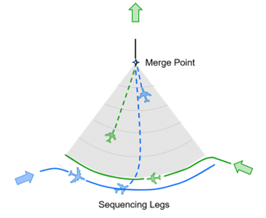
\includegraphics[width=0.6\linewidth,height=\textheight,keepaspectratio]{./figures/Point Merge Structure.png}

}

\caption{\label{fig-point-merge}Point-merge overview}

\end{figure}%

The Point Merge System has been successfully implemented at various
airports worldwide, demonstrating its effectiveness in enhancing
airspace efficiency and reducing the environmental impact of fuel
consumption. In Brazil, Guarulhos International Airport (SBGR) --- one
of the busiest hubs in Latin America --- faces daily challenges related
to high traffic density. To address these issues, PMS was implemented
for arrival procedures at SBGR in May 2021. With a recent deployment in
2024, PMS was introduced at Lisbon Airport (LPPT). The following is an
illustration of flight trajectories at SBGR and LPPT during periods
before and after the implementation of the Point Merge System (PMS).

\begin{figure}[H]

\centering{

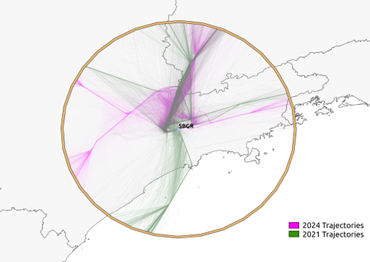
\includegraphics[width=0.7\linewidth,height=\textheight,keepaspectratio]{./figures/trajectory 2019_2024_SBGR.png}

}

\caption{\label{fig-pms-sbgr-2019-2024}Point-merge operations at
Guarulhos (SBGR) (2019 vs 2024)}

\end{figure}%

\begin{figure}

\begin{minipage}{0.50\linewidth}

\begin{figure}[H]

{\centering 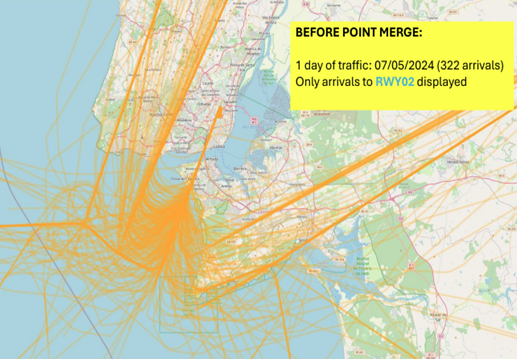
\includegraphics[width=1\linewidth,height=\textheight,keepaspectratio]{./figures/beforePMS_rwy02.png}

}

\subcaption{LPPT runway 02 - before point-merge}

\end{figure}%

\end{minipage}%
%
\begin{minipage}{0.50\linewidth}

\begin{figure}[H]

{\centering 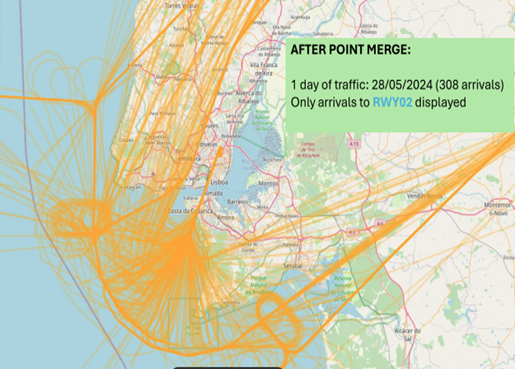
\includegraphics[width=1\linewidth,height=\textheight,keepaspectratio]{./figures/afterPMS_rwy02.png}

}

\subcaption{- post point-merge deployment}

\end{figure}%

\end{minipage}%
\newline
\begin{minipage}{0.50\linewidth}

\begin{figure}[H]

{\centering 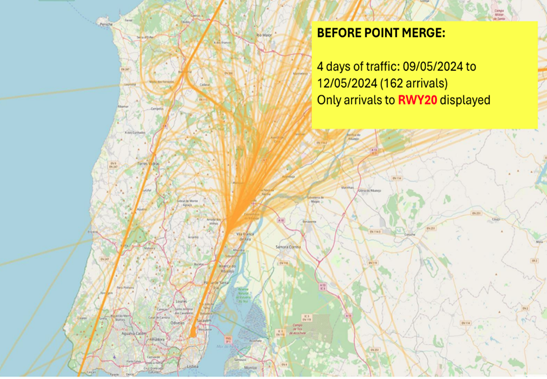
\includegraphics[width=1\linewidth,height=\textheight,keepaspectratio]{./figures/beforePMS_rwy20.png}

}

\subcaption{LPPT runway 20 - before point-merge}

\end{figure}%

\end{minipage}%
%
\begin{minipage}{0.50\linewidth}

\begin{figure}[H]

{\centering 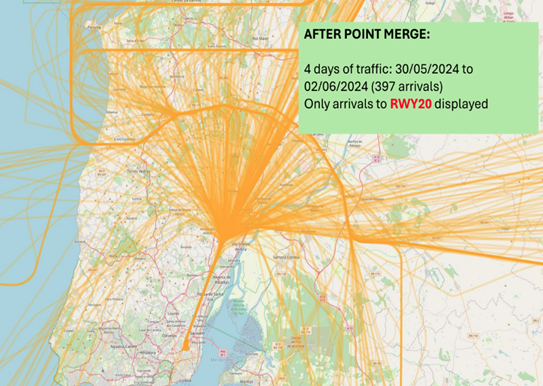
\includegraphics[width=1\linewidth,height=\textheight,keepaspectratio]{./figures/afterPMS_rwy20.png}

}

\subcaption{- post point-merge deployment}

\end{figure}%

\end{minipage}%

\end{figure}%

Monitoring Additional Time in TMA is valuable for assessing the impact
of the Point Merge System (PMS) implementation on airspace operational
performance. This indicator reflects the extra time an aircraft spends
in the TMA compared to an ideal flight profile. A comparison of KPI08
values was conducted for periods before and after the implementation of
PMS. For SBGR, the analysis covered the years 2019 (pre-PMS) and 2024
(post-PMS). These periods were chosen to avoid analytical bias, since
PMS implementation at Guarulhos took place during the COVID-19 pandemic.
The analysis period for LPPT spanned from March 2023 to July 2024. The
following graph presents the results obtained. Reference times and
additional times were calculated on a monthly basis.

\begin{figure}[H]

\centering{

\pandocbounded{
\includegraphics[keepaspectratio]{09-studies_files/figure-pdf/fig-lppt-asma-monthly-1.pdf}}

}

\caption{\label{fig-lppt-asma-monthly}Monthly evolution of the
additional time in terminal airspace in LPPT}

\end{figure}%

\begin{figure}[H]

\centering{

\pandocbounded{
\includegraphics[keepaspectratio]{09-studies_files/figure-pdf/fig-sbgr-asma-monthly-1.pdf}}

}

\caption{\label{fig-sbgr-asma-monthly}Monthly evolution of the
additional time in terminal airspace in SBGR}

\end{figure}%

The results presented in Figure~\ref{fig-lppt-asma-monthly} indicate an
increase in additional time in the arrival airspace at LPPT. The
additional time is shown for the period following the deployment of the
point merge operations covering March through August focussing on the
last 40NM around Lisbon. The results are also broken out to showcase the
behaviour for both landing directions at Lisbon, i.e., runway 02 and
runway 20. For both runways, an increase in the additional time can be
observed. Aside the results for March that represents the transition to
point merge operations, the observed additional time increased on
average by about a minute when compared to the pre-deployment year 2023.
It must be noted that the results for LPPT are point-in-time snapshots
and influenced by the start of operations. There might be additional
flow control measures in place to support the transition, including
additional buffers or alignment patterns. Future work could explore how
the actual arrival routes changed based on the newly arrival management
technique.

The operations at SBGR show a clear trend when comparing pre-pandemic
traffic levels to the current arrival flows, c.f.
Figure~\ref{fig-sbgr-asma-monthly}. A mild seasonal pattern is
observable, with the monthly average additional time in terminal
airspace ranging post the point-merge implementation lower than in 2019.
With the summer months a more varied behaviour is observed seen a
fluctuation of the observed additional times.

For the implementation of the PMS, the following observations can be
made. Operationally, the PMS enabled a higher occupancy rate within the
terminal airspace. By design, the PMS enhances the terminal's capacity
to manage and organise inbound traffic more efficiently. However, the
runway throughput remained unchanged, as increasing runway capacity
would require physical infrastructure modifications or change of the
operational concept (i.e., separation minima). Consequently, although
the terminal airspace can now accommodate a greater number of approaches
simultaneously, the airport's ground infrastructure cannot absorb this
increased demand at the same pace. This mismatch leads to longer dwell
times within the terminal area as aircraft await clearance to land.

\section{Air Traffic Services at Curitiba and Lisbon
Continental}\label{air-traffic-services-at-curitiba-and-lisbon-continental}

\subsection{Overview Curitiba ACC}\label{overview-curitiba-acc}

The Curitiba Area Control Center (ACC-CW) is one of four Area Control
Centers strategically distributed across Brazil. Located in the city of
Curitiba, in the state of Paraná, ACC-CW plays a crucial role in
controlling the airspace of the southern region of the country, ensuring
safe and efficient operations for both civil and military aircraft.

ACC-CW's jurisdiction covers the entire portion of the Curitiba Flight
Information Region (FIR-CW), excluding the airspace delegated to the
South-east Regional Airspace Control Center (CRCEA-SE). This
jurisdiction totals approximately 1.7 million km², representing 7.7\% of
the airspace delegated to Brazil. Within this airspace, the Air Traffic
Control Service, Flight Information Service, and Alert Service are
provided.

The Air Traffic Control Service is provided to all aircraft flying above
FL 150. Additionally, this service is exclusively provided to aircraft
flying above FL 120 in CTA 2 (departures and arrivals for Viracopos
Airport in Campinas-SP) and CTA 4 (departures and arrivals for Vitória
Airport in Espírito Santo).

In 2024, traffic within FIR-CW exceeded 492,000 flights, representing a
25\% increase compared to 2023 (394,000 flights). Notably, 11 of the 30
busiest aerodromes in Brazil in 2024 are located within FIR-CW (c.f.
Figure~\ref{fig-bra-acc-tfc}).

\begin{figure}[H]

\centering{


\includegraphics[width=0.8\linewidth,height=\textheight,keepaspectratio]{09-studies_files/figure-pdf/fig-bra-acc-tfc-1.pdf}

}

\caption{\label{fig-bra-acc-tfc}Traffic figures for Brazilian ACCs}

\end{figure}%

The FIR-CW encompasses the Terminal Control Areas (TMA) of São Paulo,
Rio de Janeiro, Curitiba, Florianópolis, Porto Alegre, Foz do Iguaçu,
Campo Grande, Santa Maria, Macaé, Londrina, and Presidente Prudente. One
of the objectives of the cooperation agreement established between DECEA
and MUAC---the Rostering Philosophies and Tools Agreement---is to
support the implementation of the TOTAL ATM philosophy. ACC-CW was
selected to be the first operational unit in Brazil to implement changes
related to new philosophies and methodologies for operational staff
rostering. It was also chosen to develop and implement, with the support
of MUAC, the Air Traffic Support System for the Use of Human Resources
in Operational Needs, known as SATURNO.

The implementation of SATURNO began in March 2025 and is being carried
out in phases, with completion expected by the end of the year. To
improve planning for operational position configurations and the
allocation of air traffic controllers during shifts, the ACC-CW
airspace, currently, is divided into 18 sectors and two regions: North
and South.

\begin{figure}[H]

\centering{

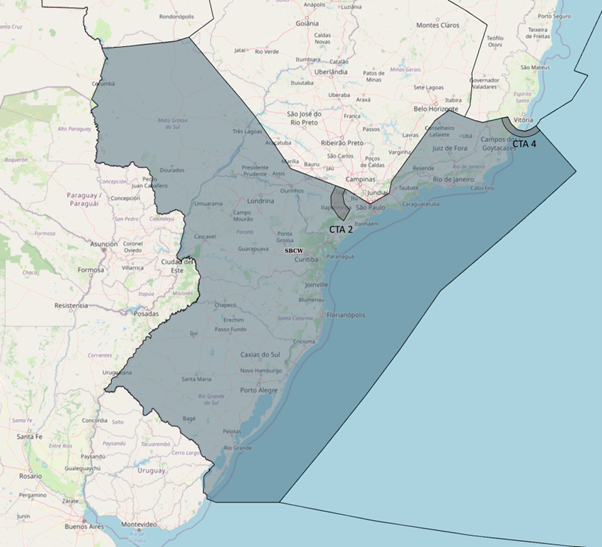
\includegraphics[width=0.8\linewidth,height=\textheight,keepaspectratio]{./figures/acc_ctb_northsouth.png}

}

\caption{\label{fig-ctb-northsouth}ACC-CW area of responsibility}

\end{figure}%

\subsection{Center-level comparison Curitiba ACC and Lisbon
Continental}\label{center-level-comparison-curitiba-acc-and-lisbon-continental}

\begin{figure}[H]

\centering{

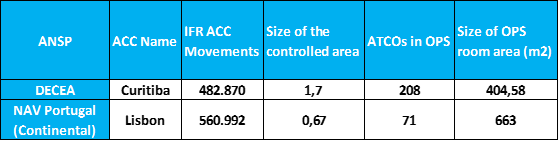
\includegraphics[width=0.98\linewidth,height=\textheight,keepaspectratio]{./figures/comp_acc.png}

}

\caption{\label{fig-HLC-Curitiba-Lisbon}High-level comparison ACC
Curitiba and Lisbon}

\end{figure}%

In light of this report Figure~\ref{fig-HLC-Curitiba-Lisbon} provides an
initial side-by-side comparison between DECEA and NAV Portugal
(Continental) regarding selected operational characteristics of their
Area Control Centers (ACCs). While each organisation operates within its
own regional and structural context, some key characteristics are worth
highlighting.

Despite operating within a smaller controlled airspace, NAV Portugal
managed a higher volume of IFR ACC movements than DECEA during the same
period while handling nearly 25\% fewer flight hours. This points to a
denser and more concentrated traffic environment, likely driven by
Portugal's geographical location within Europe and the structure of its
flight corridors.

Another relevant aspect is the number of air traffic controllers (ATCOs)
assigned to the operations room. NAV Portugal handles its operational
workload in a larger OPS room with only 71 ATCOs, highlighting distinct
differences in operational concepts, levels of automation, and staffing
philosophies between the two organizations.

In terms of sector configuration, Curitiba operated up to 13 sectors at
the end of 2024, compared to a maximum of 9 sectors in Portugal. For the
year as a whole, the total number of sector hours was similar, with
Portugal recording approximately 2,000 more hours.

This characterisation underscores the importance of accounting for
regional characteristics and operational context when interpreting air
navigation service metrics or designing systems such as staffing models
or control room layouts. It will be interesting to expand this initial
topic study by addressing the traffic characteristics on the basis of
trajectory, flow and sequencing measures applied to handle the traffic
within the respective areas of responsibility. This will support a
refined assessment of the performance benefits from the implemented
concept of operations.

\section{Summary}\label{summary-5}

This chapter highlighted two topics of interest for both parties. It
offers a first insight into operational concepts, their implementation,
and observed performance benefits.

Point merge is a sequencing technique that gained higher visibility over
the past years. This initial comparison comprises a snapshot at the
system deployed at SBGR and - a recent implementation at - LPPT.

Both groups are interested in advancing the state-of-the-art in
assessing network- and center-level aspects. To move towards a more
granular comparison, this report showcases two broadly comparable air
traffic service units in Brazil and Europe. The comparison allowed for a
high-level comparison on a set of harmonised indicators suitable to
describe the scope of the service provision. This was useful to
characterise the similarities and differences between both units. Future
work will revolve around addressing the operational aspects within the
respective areas of responsibility and deployed operational flow and
sequencing concepts.

\bookmarksetup{startatroot}

\chapter{Conclusions}\label{conclusions}

This fourth edition of the Brazil-Europe operational ANS performance
comparison report builds on the joint project between the Performance
Section of DECEA and the Performance Review Unit of EUROCONTROL. The
collaboration aims at fostering the understanding and support the
further development of approaches to measure operational performance in
both regions. This report builds on a subset of indicators and metrics
established under the umbrella of ICAO's Global Air Navigation Plan ICAO
(2019b). The work is also used to showcase the application of the GANP
indicators within a bi-regional and multi-regional project. DECEA and
EUROCONTROL engage actively within the international community and share
their findings of their joint bi-regional work.

This iteration also comprised the integration of additional data source
and topics. A first characterisation of the different networks was
introduced, and two additional topics studied. The new data sources
offer to perform more fine-grained analyses of the observed operational
efficiency performance. This will allow to further develop and
complement the framework. The report also identified several
observations and ideas for future research which pave the way ahead for
augmenting the associated set of comparison analyses.

This report kicked off by examining the commonalities and differences in
terms of the organisation of air navigation services in both regions.
This was complemented by investigating the air traffic demand to better
understand the factors influencing operational performance. The air
navigation service provision is less fragmented in Brazil than in
Europe. This plays out in the total number of air traffic service units.
Both regions operate a central flow management function to ensure
network wide flow management.

In terms of air traffic demand, both regions were impacted by the
unprecedented decline of air traffic. Regional and global traffic
restrictions resulted in different patterns. With Europe zooming in on
pre-pandemic traffic levels and Brazil consistently ranging above the
pre-pandemic traffic, this report also marks the new reference for
future iterations. Both regions - while having their separate challenges
- have certainly completed the pandemic phase. The traffic situation is
also reflected by the demand at the study airports. There is also a
higher level of diversity in terms of air traffic evidenced by the share
of light types serviced at the comparison airports. International
traffic is more centralised in Brazil than in Europe.

The observed punctuality in both regions was strongly influenced by the
prevailing network effects. Particularly, Europe suffered strongly from
the impact of two years of record ATFM delays that further rippled down
and amplified local constraint issues. This is evidenced by the high
share of departure delays. The reactionary knock-on effect amplified
further the overall punctuality performance.

The utilisation of available runway system capacities is a fundamental
enabler for high levels of operational performance. This report showed
that associated capacities are commensurate with the current traffic
levels. For the majority of airports, the realised throughput ranges
still below the maximum declared capacities.

Operational efficiency is measured in this report in the form of the
additional time during the surface movement phases and the terminal
arrival phase. On average, taxi-in operations are less constrained than
taxi-out operations. The observed performance varies across the airports
and timeframe. In terms of arrival management, air traffic in Brazil
observed higher additional times in the terminal airspace. This report
showed that the scale effect of lower air traffic is potentially masked
by the effects of airspace redesign in Brazil. In the European region,
it appears that the higher level of air traffic demand puts pressure on
the arrival management and sequencing, and 2022 marks a return to higher
additional times within the terminal airspace. Further research can help
to identify drivers and performance enablers.

The joint work also helped to promote the approach and state-of-the-art
with the international community. Both groups are contributing to the
ICAO GANP Performance Expert Group and the multi-national Performance
Benchmarking Working Group. The wider harmonisation of performance
related data and joint refinement of the guidance material and
application of the performance framework start paying dividends. For
example, PBWG concluded in its most recent meeting to collaborate on
topics of mutual interest for which this report supported the initial
research and validation.

A further outcome of the project is the close technical collaboration.
It is planned to augment the report and its future editions with a
rolling web-based monitoring, including regular updates of the
underlying data. This and future reports will help to complement the
time series of the measures tracked.

\bookmarksetup{startatroot}

\chapter*{References}\label{references}
\addcontentsline{toc}{chapter}{References}

\markboth{References}{References}

\phantomsection\label{refs}
\begin{CSLReferences}{1}{0}
\bibitem[\citeproctext]{ref-apdf_v1_2019}
EUROCONTROL. 2019. {``Eurocontrol {Specification} for {Operational ANS
Performance Monitoring} - {Airport Operator Data Flow}.''}
\url{https://www.eurocontrol.int/publication/eurocontrol-specification-operational-ans-performance-monitoring}.

\bibitem[\citeproctext]{ref-CODA-2023}
EUROCONTROL Central Office of Delay Analysis. 2023. {``All-Causes Delays
to Air Transport in Europe, Annual 2022.''}
\url{https://www.eurocontrol.int/publication/all-causes-delays-air-transport-europe-annual-2022}.

\bibitem[\citeproctext]{ref-icao_doc9750_2019}
ICAO. 2019b. \emph{Doc 9750, {Capacity} \& {Efficiency}, {Global Air
Navigation Plan} 2016-2030}. Sixth Edition. {Montreal, Canada}:
{International Civil Aviation Organization}.

\bibitem[\citeproctext]{ref-icao-doc-9750-2019}
ICAO. 2019a. \emph{Doc 9750, Capacity \& Efficiency, Global Air
Navigation Plan 2016-2030}. Sixth Edition. Montreal, Canada:
International Civil Aviation Organization.

\end{CSLReferences}

Eurocontrol. (2014). Point Merge: Integration of Arrival Flows Enabling
Extensive RNAV Application and Continuous Descent. Eurocontrol
Experimental Centre.

FRANZINI, Bruno Monteiro et al.~(2024). Analysis of Guarulhos Point
Merge Adherence Based On Additional Time In Tma And Trajectory
Clustering.. In: Anais do XXI Simpósio de Transporte Aéreo - SITRAER
2024.

ICAO. (2016). Continuous Descent Operations (CDO) Manual. International
Civil Aviation Organization.




\end{document}
